% !TEX TS-program = xelatex
% !BIB TS-program = bibtex
\documentclass[12pt,letterpaper]{article}
\usepackage{fontspec}
% Preserve the course style when its optional code font is unavailable.
\IfFontExistsTF{Fira Code}{}{%
  \defaultfontfeatures[Fira Code]{UprightFont=lmmono10-regular.otf}}
% Captions: same font as the body, smaller and italic, with a bold label.
% All captions (figures and tables) go below the float.
\usepackage{caption}
\captionsetup{font={footnotesize,it}, labelfont={bf,up}, labelsep=period,
  justification=justified, singlelinecheck=false, skip=6pt}
\usepackage{style/dsc180reportstyle}
% The course style puts table captions on top; put them below instead.
\floatstyle{plain}
\restylefloat{table}
% Visible, dark-blue cross-reference links (Figure 3, Table 2, Section 3.1)
\definecolor{LinkBlue}{rgb}{0.0,0.25,0.65}
\hypersetup{colorlinks=true, linkcolor=LinkBlue, citecolor=LinkBlue,
  urlcolor=LinkBlue}
% More space around floats so they separate from the text
\setlength{\textfloatsep}{18pt plus 2pt minus 4pt}
\setlength{\floatsep}{14pt plus 2pt minus 2pt}
\setlength{\intextsep}{16pt plus 2pt minus 4pt}
\raggedbottom
\widowpenalty=10000
\clubpenalty=10000

\title{Neural Network Surrogates for TGLF: Prediction Accuracy and Uncertainty}
\author{Ryan Lindberg \And
  Sweekrit Bhatnagar \And
  Joseph Calderon \And
  Aryan Nath \AND
  {\normalfont Mentors: Emily Belli, Jeff Candy, and Igor Sfiligoi}}
% Confirm author spelling, order, and mentor attribution before submission.

\begin{document}
\maketitle
\begin{center}
  \small Quarter 1 checkpoint draft
\end{center}

\begin{abstract}
  Repeated runs of the gyrokinetic code CGYRO and the trapped gyro-Landau
  fluid (TGLF) transport model can be costly. This project
  investigates methods for approximating the ion heat, electron heat, and electron
  particle fluxes predicted by TGLF.
  We explore a variety of TGLF simulation runs, compare candidate models, and test
  choices in input representation, network design, and training to produce a machine learning model comparable to TGLF.
  An initial study of 43 scan cases shows that greater model flexibility does not consistently
  improve prediction and that low aggregate error can coexist with incorrect
  flux signs. A comparison on a larger parameter-scan database shows that a five-network
  ensemble performs best among the modeling techniques, reducing test root mean squared error
  by 59.6\%--77.2\% relative to a linear baseline across the three outputs. A controlled
  activation comparison also reveals different tradeoffs for heat and particle flux prediction.
  However, uncertainty analysis shows that the accuracy of the neural network ensemble depends
  heavily on the TGLF data it is trained on. Test data with variables outside the range of the
  training data, or even data from the DIII-D tokamak that is not distributed like the training data, is subject
  to significant accuracy drops, usually through a systematic bias in flux predictions. Overall,
  this motivates further development and tuning through a larger variety of training data and
  continued robust uncertainty analysis.
\end{abstract}

\begin{center}
  Code: \url{https://github.com/lindbergryan04/dsc180a-project-1}
\end{center}

\section{Introduction}
\subsection{Problem Statement and Research Question}

Turbulence transports heat and particles across a tokamak plasma and affects
its temperature and density profiles. Predicting these fluxes is part of
modeling plasma confinement. Detailed turbulence simulations are expensive,
and even reduced models such as the trapped gyro-Landau fluid (TGLF) model
can become costly when a larger
calculation requires many evaluations \citep{meneghini2017, cao2026}.
A surrogate learns to approximate a simulation from previously computed
input-output pairs, making repeated predictions less expensive.

Our research question is which modeling approaches and design choices provide
useful approximations of TGLF under the available data and computational
constraints. We began by examining the plasma inputs, output scales, and data
quality, then explored regression, tree-based, and neural network methods.
We assess choices through prediction error, computational cost, and behavior
across plasma conditions. Uncertainty estimates provide an additional way to
examine model reliability. One case study uses plasma conditions from
\href{https://www.ga.com/magnetic-fusion/diii-d}{DIII-D}, a tokamak operated
by General Atomics in San Diego. A tokamak uses magnetic fields to confine
hot plasma in a doughnut-shaped chamber. We use inputs based on a DIII-D
experiment to compare surrogate predictions with TGLF outputs.

The prediction targets are ion heat flux $Q_i$, electron heat flux $Q_e$, and
electron particle flux $\Gamma_e$. The reference values are TGLF outputs.
Agreement with these values measures approximation of TGLF; it does not by
itself establish agreement with experimental measurements or nonlinear
gyrokinetic simulations. This checkpoint reports an exploratory comparison on
a small scan dataset and a more developed neural network study on a larger
database. The distinction between these experiments matters when interpreting
which methods performed well.

\subsection{Related Work on Neural Network Transport Surrogates}

\citet{meneghini2017} developed neural network surrogates for TGLF and for
EPED1, a model of the plasma edge pedestal, and incorporated them into a coupled core and pedestal modeling workflow.
Their TGLF architecture description in Section~3.1 specifies an ensemble of
32 independently initialized networks, each with one hidden layer of 60
neurons. This provides a precedent for averaging networks and a reference
for investigating ensemble size. It does not establish an optimal member
count for our data. Our deeper network architecture and training database
differ from theirs, so our experiments evaluate the approach in a different
setting.

Model evaluation also requires attention to local behavior.
\citet{vandeplassche2020} developed the QuaLiKiz neural network (QLKNN)
to approximate QuaLiKiz, a quasilinear gyrokinetic transport model. Their work emphasizes evaluating local transport
behavior alongside aggregate prediction error, motivating our checks of flux
trends and individual prediction failures.
\citet{cao2026} developed a wavenumber-informed neural network for TGLF
(TGLF-WINN) using feature engineering, transformed
flux targets, and supervision of flux contributions at individual
wavenumbers. Their comparisons of individual design components illustrate
how controlled experiments can identify useful modeling choices. We use
integrated flux targets and test simpler representations and network choices;
we do not implement their wavenumber supervision in the experiments reported here.

Training data selection is another direction in this literature.
\citet{zanisi2024} introduced Active Deep Ensembles for Plasma Turbulence,
using neural network ensembles to guide training-data selection for QuaLiKiz
surrogates. This provides context for studying data requirements and
uncertainty, although our current experiments use fixed training datasets
rather than active acquisition. Finally, \citet{dudding2022} developed the
third version of the TGLF saturation rule (SAT3) using nonlinear
simulations with the gyrokinetic code CGYRO, with particular
attention to isotope dependence. The course's starter dataset draws on that
work, but the added TGLF outputs supplied for our analysis use the second
version of the saturation rule (SAT2). The
saturation rule and reference simulation must therefore remain explicit.

\subsection{Datasets: Starter Scans, \texttt{scan\_db}, and Evaluation Sets}

The starter dataset contains 43 plasma cases arranged in controlled scans
around a reference condition. Case names identify 26 letter groups and an ion
isotope. Eight groups contain complete hydrogen, deuterium, and tritium
triplets. Some inputs change together: for example, the electron and ion
temperature gradients are equal in these cases. These dependencies limit the
separate effects that can be inferred from correlations. We retained all 43
cases after basic validity checks, including cases flagged for further review.

The larger \texttt{scan\_db} dataset contains 5,000 TGLF cases with multiple
inputs varied simultaneously over prescribed ranges. The sampled continuous
coordinates use uniform distributions, with collision
frequency sampled logarithmically. Unlike the starter scans, electron and ion
temperature gradients vary independently. Each case supplies a complete input
listing in \texttt{input.tglf.gen} and species-resolved fluxes in
\texttt{out.tglf.gbflux}. We retain the supplied gyro-Bohm normalization and
the sign of particle flux.

Additional supplied data support focused checks. The
\texttt{scan\_db\_outside} collection contains nine groups of 30 cases, each
placing one input outside its training range. The \texttt{data\_d3d}
collection includes 300 TGLF evaluations with perturbed inputs around a
DIII-D reference condition. These serve as evaluation cases in the uncertainty
study; they are distinct from the new DIII-D training database described in
the remaining work.

Each of the nine \texttt{scan\_db\_outside} groups sweeps exactly one input
strictly beyond the range it was sampled from in \texttt{scan\_db}, while
holding every other input inside its nominal training range
(Table~\ref{tab:ood-sweeps}). This design isolates extrapolation along one
coordinate at a time instead of the joint extrapolation that an arbitrary new
input vector could produce.

\begin{table}[htbp]
  \centering
  \small
  \begin{tabular}{llll}
    \toprule
    Group                      & Varied input          & Training range & Outside range \\
    \midrule
    \texttt{ood\_RLTS\_1}      & $R/L_{Te}$             & 1.5--3.5        & 3.5--5.0       \\
    \texttt{ood\_RLTS\_2}      & $R/L_{Ti}$             & 1.5--3.5        & 3.5--5.0       \\
    \texttt{ood\_RLN}          & $R/L_{n}$              & 1.0--3.0        & 3.0--4.5       \\
    \texttt{ood\_TAUS\_2}      & $T_i/T_e$              & 0.5--1.5        & 1.5--2.5       \\
    \texttt{ood\_XNUE}         & $\nu_{ei}$             & 0.01--1.0       & 1.0--5.0       \\
    \texttt{ood\_Q\_LOC}       & $q$                    & 1.5--2.5        & 2.5--4.0       \\
    \texttt{ood\_KAPPA\_LOC}   & $\kappa$               & 1.0--2.0        & 2.0--2.5       \\
    \texttt{ood\_DRMAJDX\_LOC} & $\Delta'$              & $-0.5$--0.0     & $-0.75$--$-0.5$ \\
    \texttt{ood\_RMIN\_LOC}    & $r/a$                  & 0.25--0.75      & 0.75--0.90     \\
    \bottomrule
  \end{tabular}
  \caption{The nine \texttt{scan\_db\_outside} single-parameter
    out-of-distribution sweeps. Each group varies only the listed input beyond
    its \texttt{scan\_db} training range, holding the remaining ten inputs
    inside their nominal ranges.}
  \label{tab:ood-sweeps}
\end{table}

A separate 1,000-case DIII-D database was also generated, independent of
\texttt{data\_d3d}, following the mentor-prescribed recipe with a
member-specific seed of 4. Cases are distributed evenly across the 13
supplied radii ($r/a = 0.20$ to $0.80$). At each radius, five inputs are
perturbed from the supplied baseline profile by independently sampled
multiplicative factors: $a/L_{Te}$ and $a/L_{Ti}$ each by a separately drawn
factor in $[0.6, 1.4]$, the shared density-gradient scale $a/L_n$
(applied equally to both species) by a factor in $[0.6, 1.4]$, the
temperature ratio $T_i/T_e$ by a factor in $[0.75, 1.25]$, and the collision
frequency $\nu_{ei}$ by a factor in $[0.5, 2.0]$ drawn uniformly on a
$\log_{10}$ scale. All magnetic geometry parameters are held fixed at the
exact DIII-D equilibrium values for that radius. As of this checkpoint, TGLF
had completed 52 of the 1,000 generated cases; the remaining simulations were
still running at submission time, so this database is not yet used for
training.

\subsection{Summary of Findings and Report Roadmap}

On the 43 starter scans, greater model flexibility did not consistently
improve prediction, and low aggregate error coexisted with wrong flux signs.
On the larger \texttt{scan\_db} database, a multilayer perceptron (MLP) had the lowest error and the
fastest prediction of the models we compared, and the accuracy ensemble
reduced test root mean squared error (RMSE) by 59.6\%--77.2\% relative to a linear
baseline. The quantile ensemble's 90\% intervals covered 94--98\% of test
cases and were widest where training data was sparse. Error rose on inputs
outside the training range, and at the DIII-D reference case the surrogate
predicted higher fluxes than TGLF did.

Section~\ref{sec:methods} describes the data preparation and each model
(Table~\ref{tab:models}). Section~\ref{sec:accuracy-results} reports accuracy
and Section~\ref{sec:uncertainty-results} reports uncertainty and
outside-range behavior. Section~\ref{sec:discussion} covers limitations and the
planned DIII-D study.

\section{Methods}
\label{sec:methods}

Several models appear in this report. Table~\ref{tab:models} gives the name
used for each, what it is, and where it is described and reported. The
accuracy, quantile, and 15-network ensembles are separate experiments with
separate training runs, so their results should not be mixed.

\begin{table}[htbp]
  \centering
  \small
  \setlength{\tabcolsep}{4pt}
  \begin{tabular}{@{}p{0.2\linewidth}p{0.44\linewidth}p{0.14\linewidth}p{0.17\linewidth}@{}}
    \toprule
    Name                    & What it is                                                                                                          & Described                        & Reported                                                   \\
    \midrule
    Starter-scan models     & Mean baseline, linear, spline, quadratic, and random forest fits on the 43 starter cases                            & \S\ref{sec:starter-methods}      & \S\ref{sec:starter-results}                                \\
    Model-family comparison & Random forest, extreme gradient boosting (XGBoost), and a single MLP, each on raw and log targets, trained on \texttt{scan\_db}                 & \S\ref{sec:modelfamily-setup}    & \S\ref{sec:modelfamily-results}                            \\
    Accuracy ensemble       & Five MLPs with different seeds, averaged, predicting one value per flux; includes the activation search             & \S\ref{sec:ensemble-methods}     & \S\ref{sec:ensemble-results}, \S\ref{sec:learning-results} \\
    Quantile ensemble       & Five MLPs that each predict the 5th, 50th, and 95th percentile of every flux (pinball loss), giving a 90\% interval & \S\ref{sec:interval-methods}     & \S\ref{sec:coverage-results} to \S\ref{sec:d3d-results}    \\
    15-network ensemble     & Fifteen MLPs whose intervals come from disagreement between members                                                 & \S\ref{sec:disagreement-methods} & \S\ref{sec:disagreement-results}                           \\
    \bottomrule
  \end{tabular}
  \caption{Models in this report, the name used for each, and where it is
    described and reported.}
  \label{tab:models}
\end{table}

\subsection{Data Preparation, Input Features, and Target Transforms}

We parsed one row per case, checking numeric values, species identity, and
flux-file length before assigning output labels. In \texttt{scan\_db}, we
fixed a 70\%/15\%/15\% training, validation, and test split using random seed
42. However, further analysis of our training data revealed four cases with
negative ion heat flux, a physically impossible trait in our tokamak simulation.
Since all four cases had been assigned to training, and these do not reflect
outlier values, rather real, underlying issues with the TGLF data generation, the rows were removed.
However, the remaining splits were reserved, leaving 3,496
training, 750 validation, and 750 test cases. Negative particle flux alone
was not an exclusion criterion.

The larger-dataset models use 11 inputs: separate temperature gradients, a
shared density gradient, the ion-to-electron temperature ratio, safety factor,
elongation, flux-surface shift, normalized minor radius, ion mass, logarithmic
collision frequency, and magnetic shear. We removed constant and duplicate
coordinates. Magnetic shear was reconstructed from the TGLF inputs as
\[
  \hat{s} \equiv \frac{r}{q}\frac{dq}{dr}
  = \frac{q'\,(r/a)^{2}}{q^{2}},
\]
where $q=\mathtt{Q\_LOC}$ is the safety factor, $q'=\mathtt{Q\_PRIME\_LOC}$ is
the TGLF safety-factor gradient parameter, and $r/a=\mathtt{RMIN\_LOC}$ is the
normalized minor radius. The conversion assumes $q\neq 0$.
Identifiers and other flux outputs were excluded from the predictors.

The positive heat targets span several orders of magnitude. We modeled
$\log_{10}Q_i$ and $\log_{10}Q_e$, while retaining signed $\Gamma_e$ on its
original scale. Inputs and transformed targets were standardized using
training rows only. Heat predictions were converted back to flux units before
evaluation. This transformation changes the fitting objective; improved fit
in logarithmic space need not imply lower error in original units.

\subsection{Exploratory Data Analysis on Starter Scans}

Exploratory data analysis of the starter scans reveals insights that can guide
future model development and analysis. We first consider the outputs
themselves (Figure~\ref{fig:starter-outputs}):
\begin{enumerate}
  \item The heat fluxes span more than an order of magnitude. Across the 43
        cases, ion heat flux ranges from 4.4 to 122.8 (about 28-fold) and
        electron heat flux from 2.0 to 123.2 (about 63-fold). On a logarithmic
        axis these values are spread more evenly, which is why we model the
        heat fluxes in logarithmic space.
  \item Particle flux behaves differently. It ranges from $-0.39$ to 44.5, and
        two cases have negative (inward) flux, so a logarithm cannot be
        applied. Most cases are small, with 32 of 43 below 4 and a long tail
        of larger values. We therefore keep particle flux signed on its
        original scale.
\end{enumerate}

\begin{figure}[htbp]
  \centering
  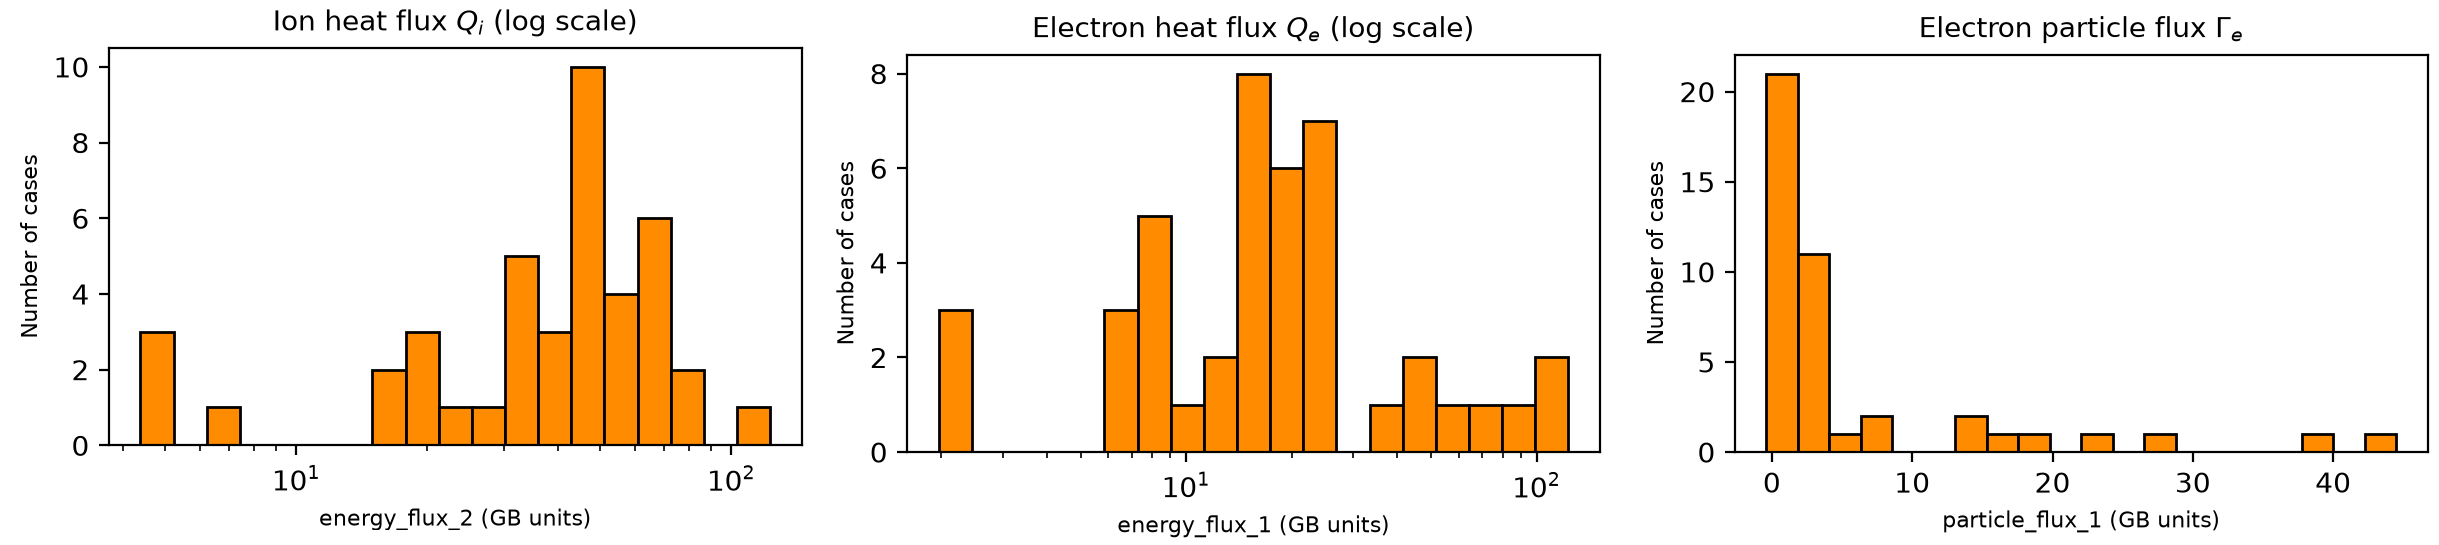
\includegraphics[width=\linewidth]{figures/starter_output_distributions.png}
  \caption{Distributions of ion heat flux, electron heat flux, and electron
    particle flux across the 43 starter cases, in gyro-Bohm units. The heat
    flux axes are logarithmic; the particle flux axis is linear and includes
    two negative values.}
  \label{fig:starter-outputs}
\end{figure}

We then analyze the inputs using the correlation heatmap in
Figure~\ref{fig:starter-corr}:
\begin{enumerate}
  \item Few inputs correlate strongly with the fluxes. The highest correlation
        with ion heat flux $Q_i$ is 0.55 (with the electron temperature
        gradient), so a single input explains only about 30\% of its variance
        in a straight-line fit. A linear model on individual inputs cannot
        approximate all of the fluxes well.
  \item Some input--output pairs are strongly correlated, such as the electron
        density gradient with electron particle flux (0.81) and with electron
        heat flux (0.75). This points to a comparatively simple dependence for
        those pairs. The starter scans change some inputs together, so these
        correlations may also reflect that coupling and should not be read as
        isolated effects.
  \item The outputs move together: $\Gamma_e$ and $Q_e$ correlate at 0.98,
        and $Q_i$ correlates with $Q_e$ at 0.80 and with $\Gamma_e$ at 0.66.
        This supports predicting the three fluxes with a shared multi-output
        model.
\end{enumerate}

\begin{figure}[htbp]
  \centering
  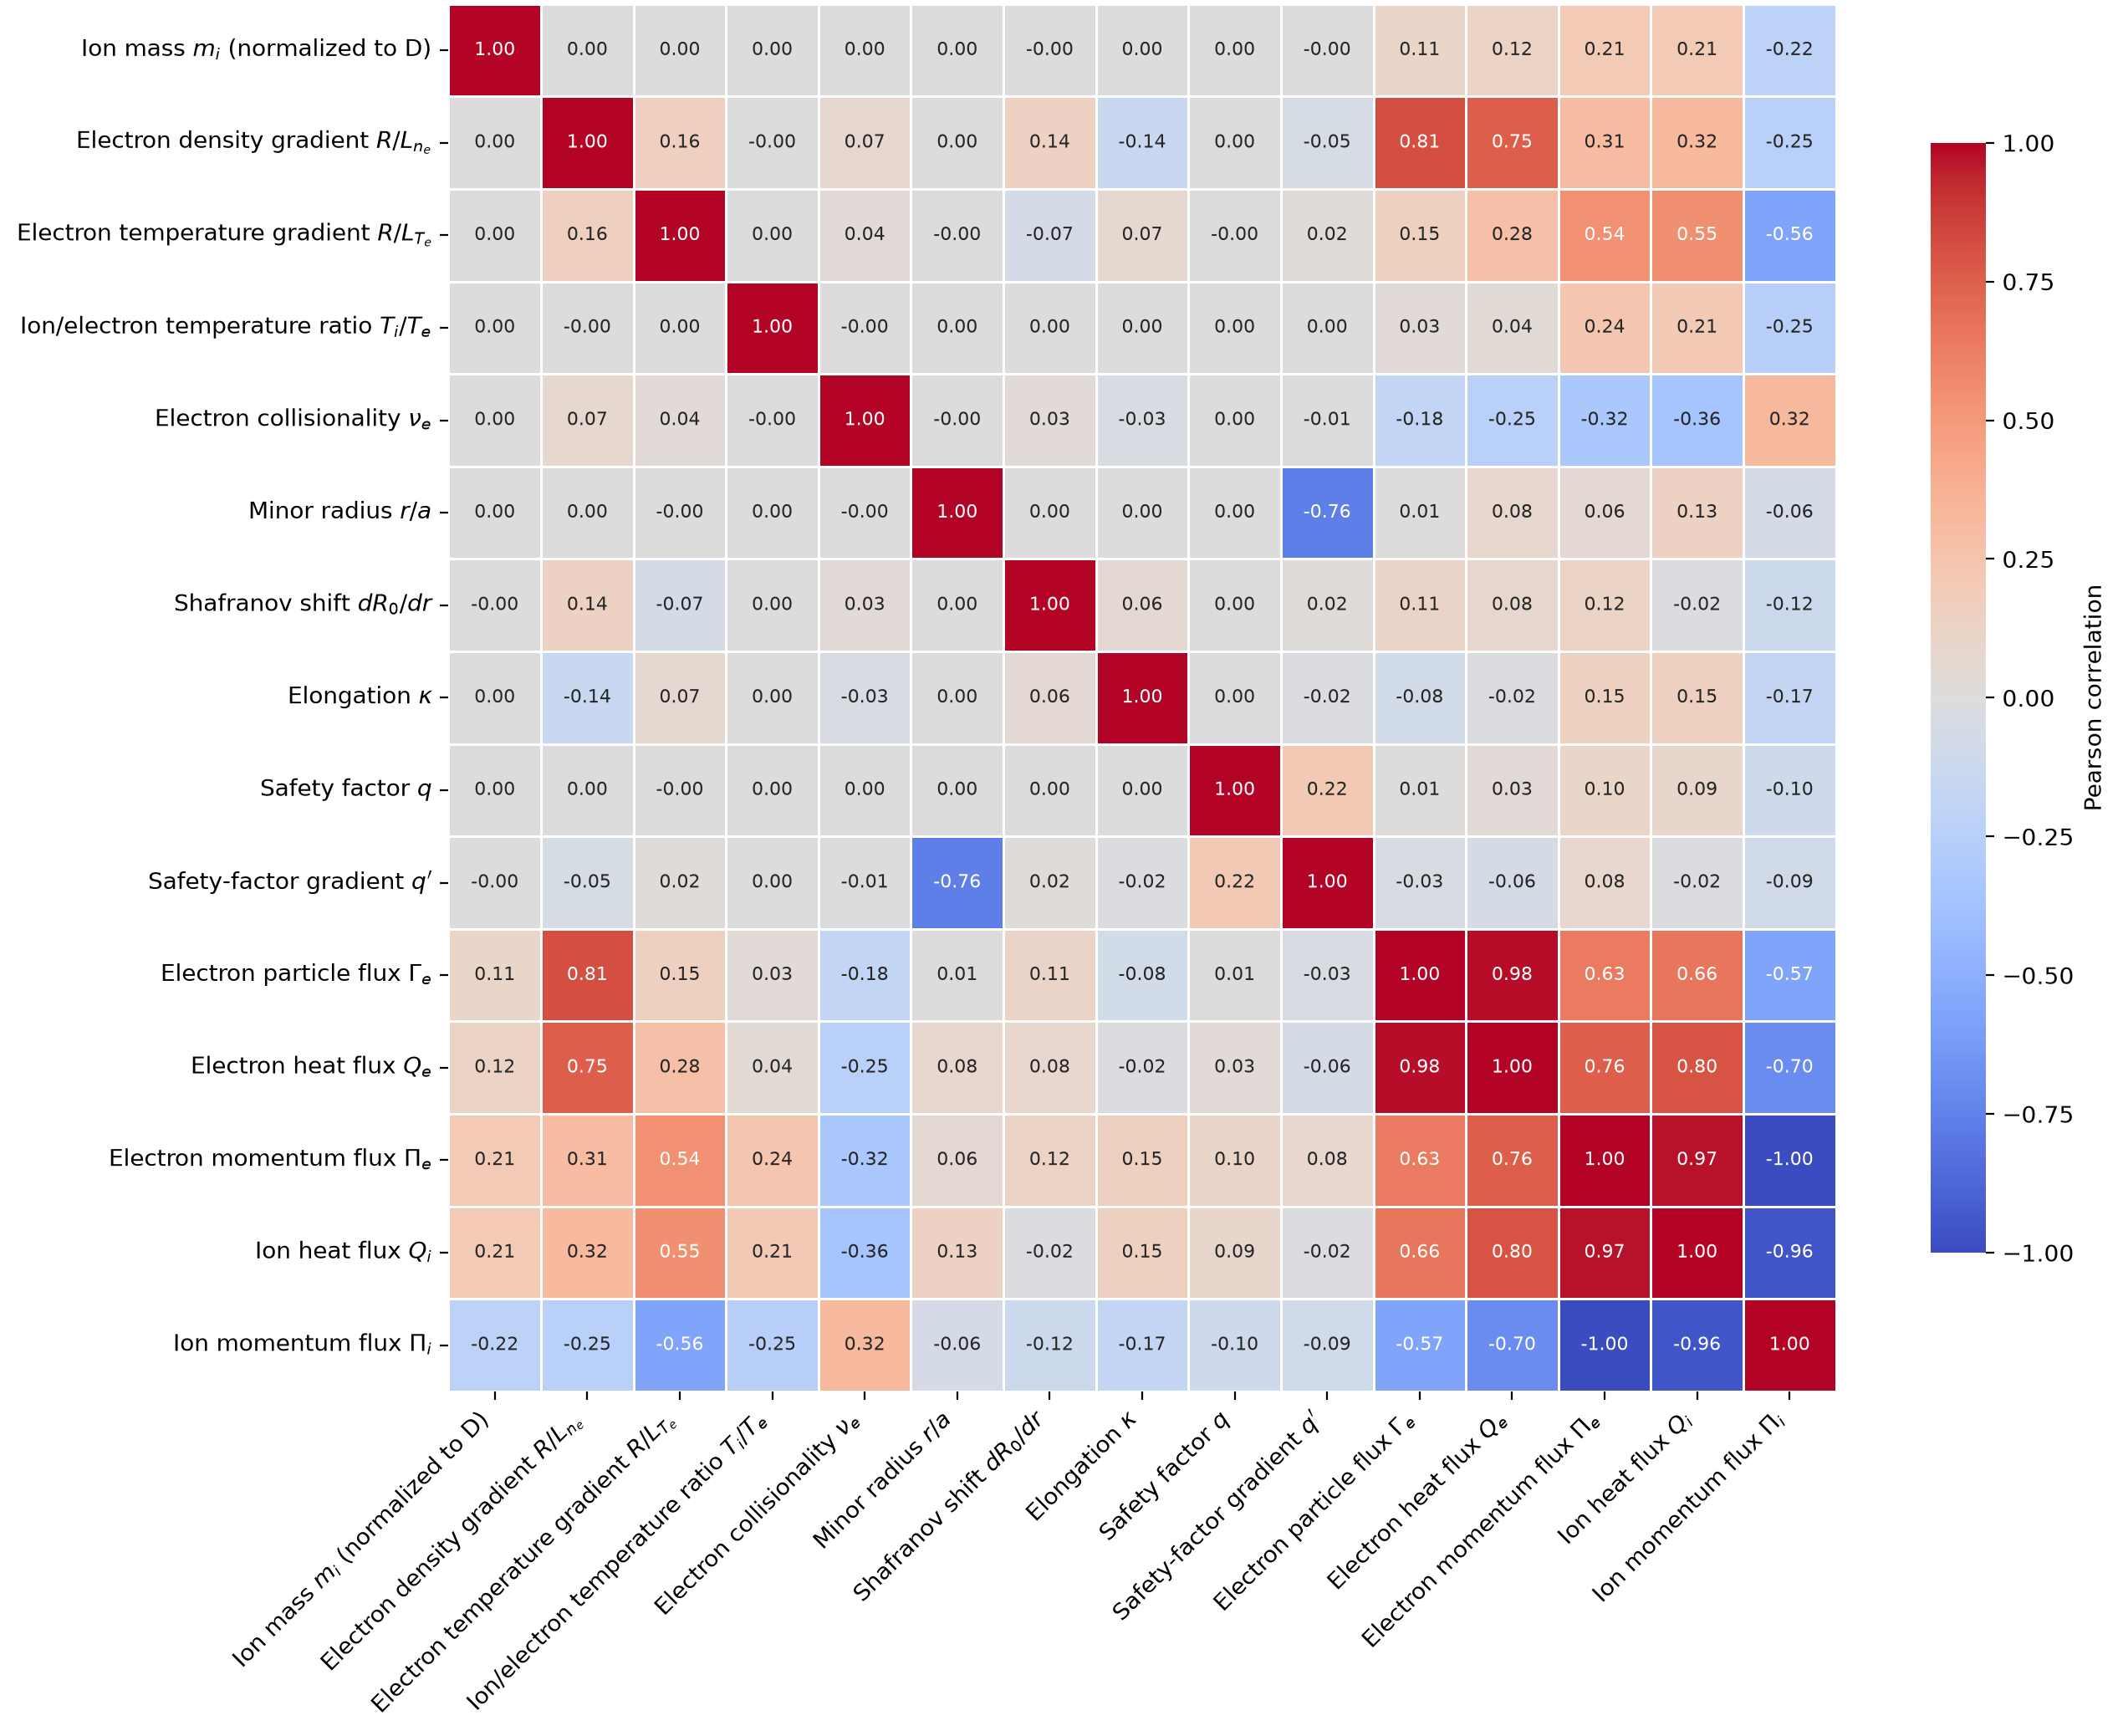
\includegraphics[width=0.85\linewidth]{figures/starter_correlation_heatmap.png}
  \caption{Pearson correlation between the inputs that vary across the 43
    starter cases and the output fluxes. Two duplicate columns
    (\texttt{RLNS\_2}, \texttt{RLTS\_2}) and \texttt{particle\_flux\_2} are
    omitted because they equal \texttt{RLNS\_1}, \texttt{RLTS\_1}, and
    \texttt{particle\_flux\_1}. Momentum fluxes are shown but are not modeling
    targets.}
  \label{fig:starter-corr}
\end{figure}

Finally, we examine how the outputs respond to individual inputs.
Figure~\ref{fig:starter-scans} illustrates why we consider nonlinear models.
Beyond the fact that we are trying to approximate complex physical
interactions inside tokamaks, we notice the following:
\begin{enumerate}
  \item The increase in output fluxes differs across input variables,
        suggesting nonlinear relationships.
  \item The faded points in many of the plots show that varying other inputs
        simultaneously changes the output flux substantially.
  \item In some cases, such as the ion temperature gradient scan, the flux
        relative to deuterium varies nonlinearly across ion species.
\end{enumerate}

\begin{figure}[H]
  \centering
  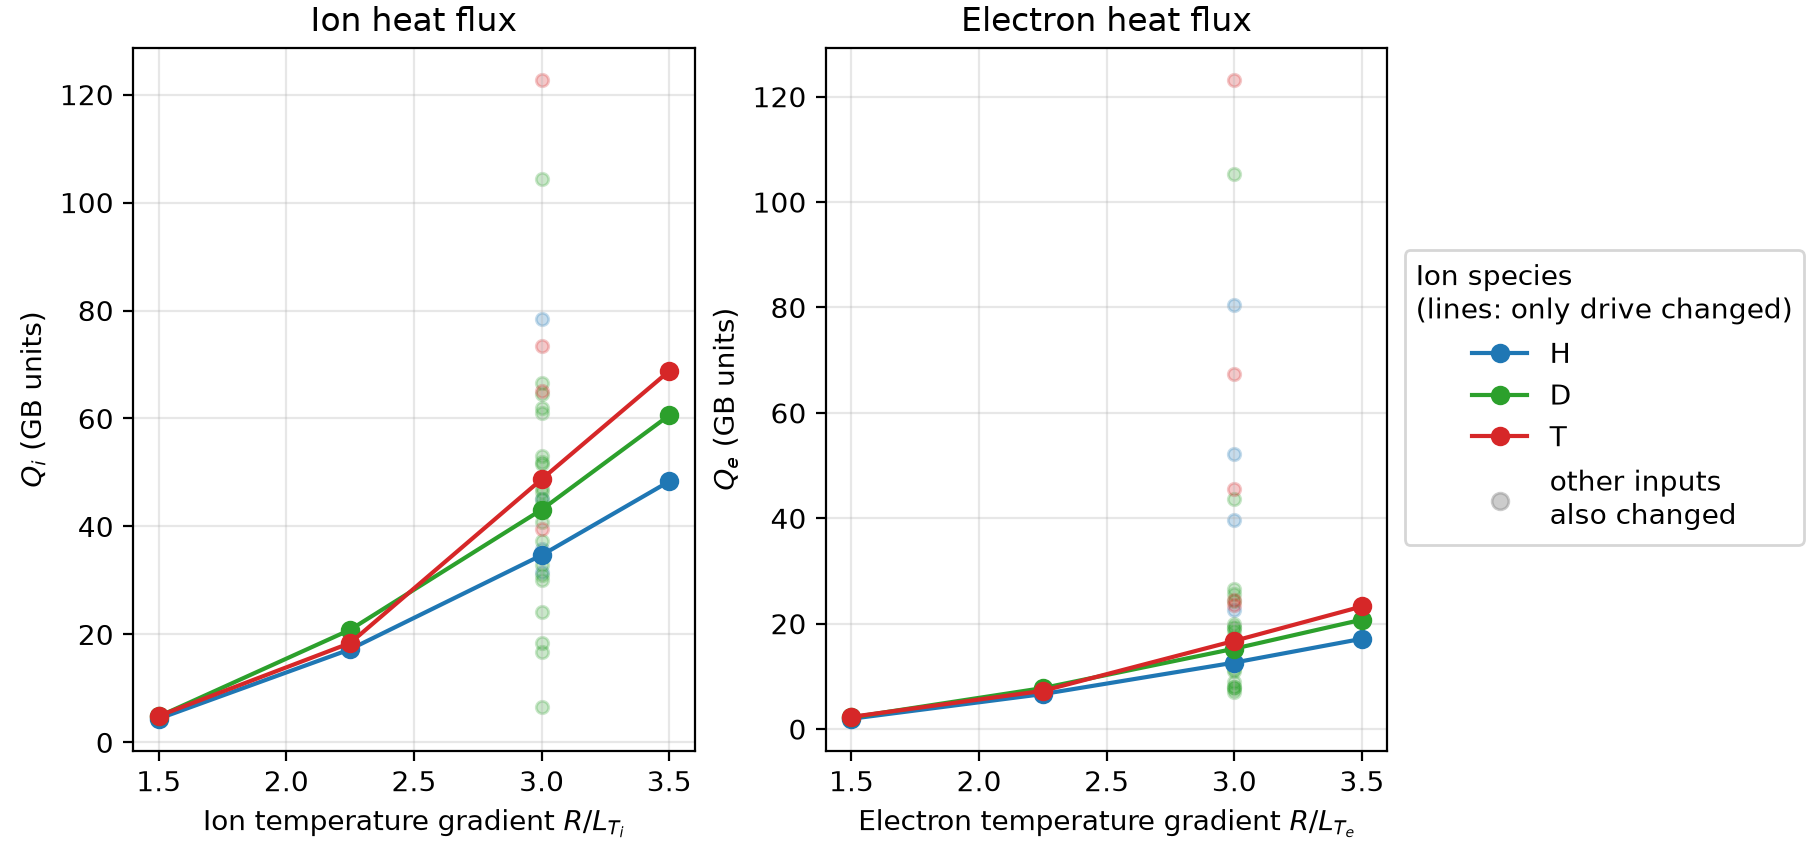
\includegraphics[width=0.7\linewidth]{figures/starter_heat_flux_gradient.png}\\[4pt]
  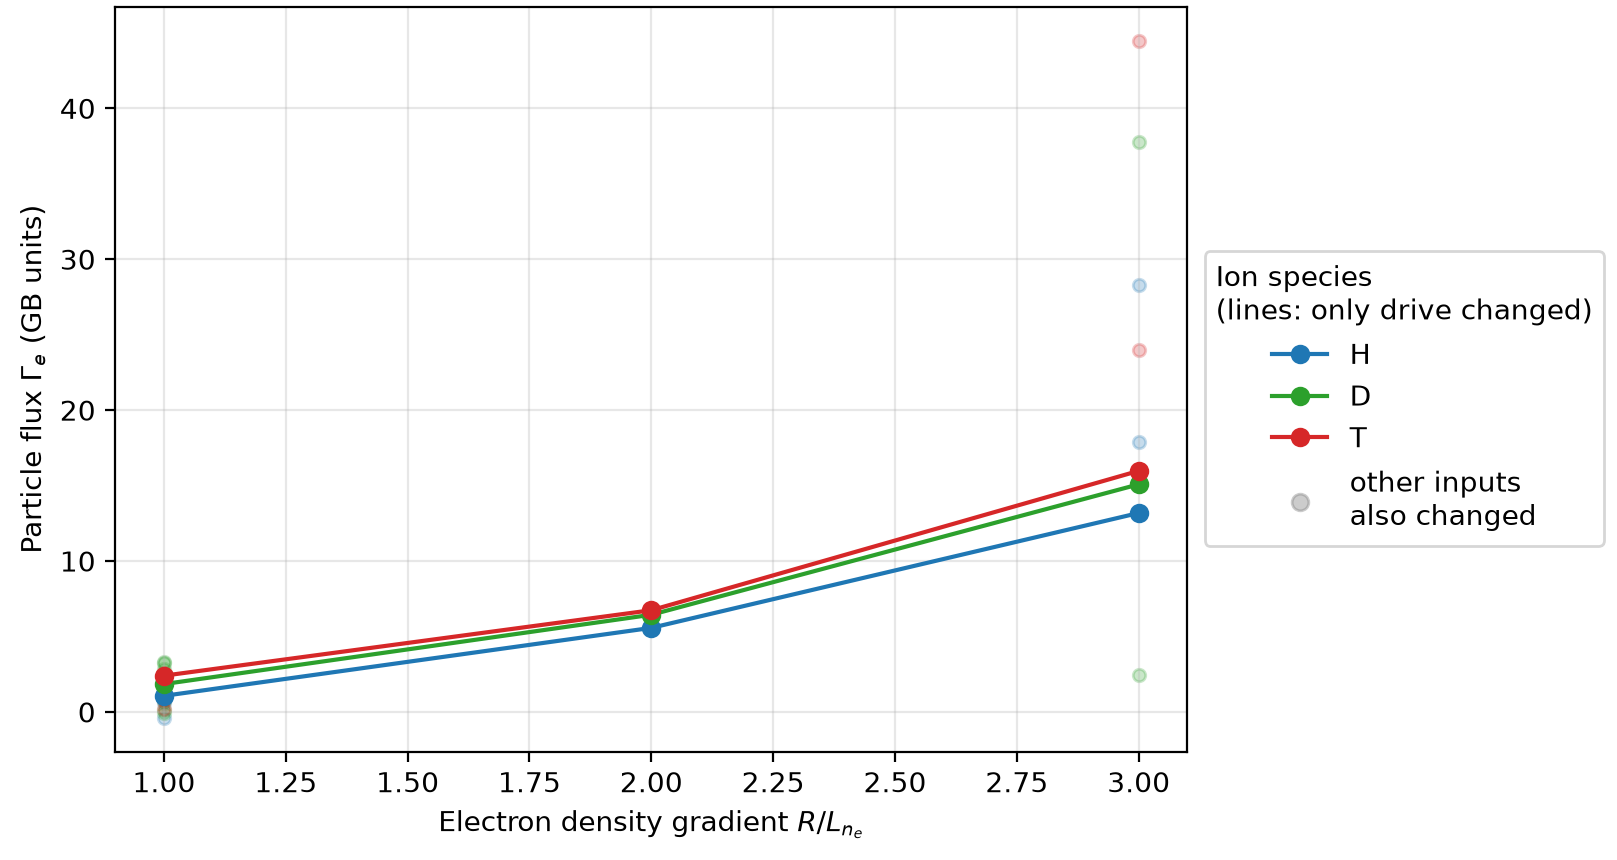
\includegraphics[width=0.42\linewidth]{figures/starter_particle_flux_density.png}\\[4pt]
  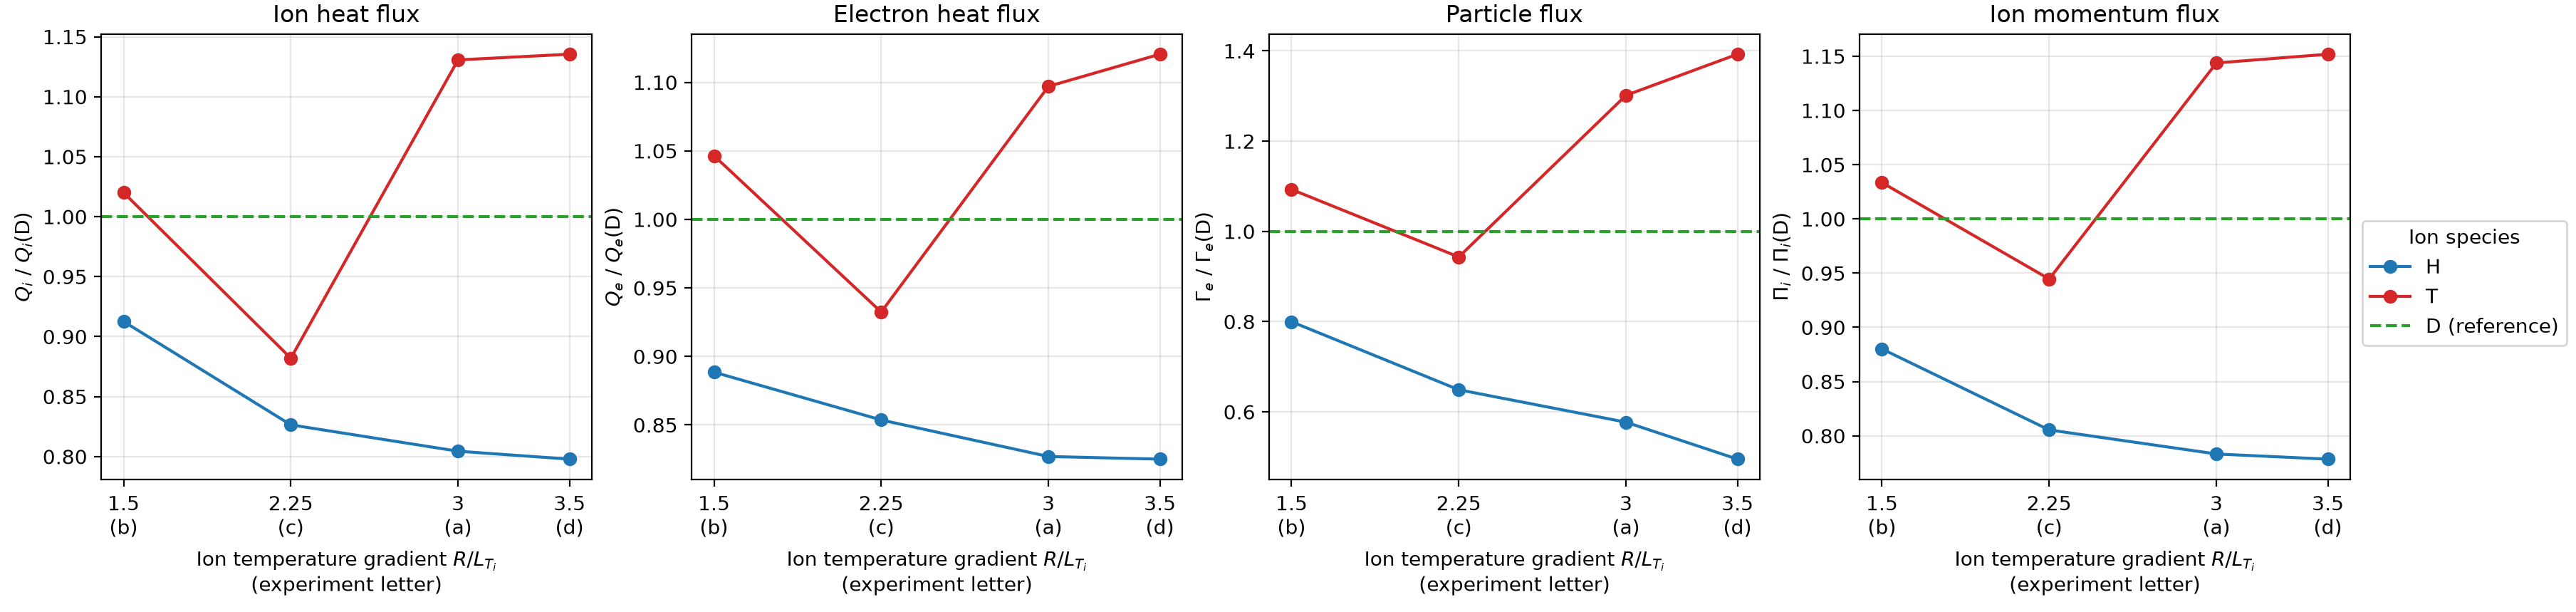
\includegraphics[width=\linewidth]{figures/starter_isotope_ratio.png}
  \caption{Starter-scan responses in gyro-Bohm units. Top: ion and electron
    heat flux against the matching temperature gradient. Middle: particle flux
    against density gradient. In both, lines join cases where only the shown
    input (and the isotope) changed, and faded points are cases where other
    inputs also changed. Bottom: hydrogen and tritium flux divided by
    deuterium flux across the ion temperature-gradient scan, labeled by
    experiment letter. These are one-at-a-time scans of three to four points
    on 43 cases, so they illustrate input interactions rather than establish
    the shape of any response.}
  \label{fig:starter-scans}
\end{figure}

\subsection{Exploratory Regression and Forest Models on the Starter Scans}
\label{sec:starter-methods}

The initial comparison used ten physical input coordinates on the 43 starter
cases, representing the tied temperature gradients with one coordinate.
We compared a training-mean baseline, linear regression variants,
additive splines, quadratic terms with interactions, and a random forest.
The variants tested logarithmic collision frequency and, for heat fluxes,
logarithmic targets. The forest used 100 trees, maximum depth four, and a
minimum leaf size of three.

For outer evaluation, we held out one entire letter group at a time, keeping
related isotope cases together. Inner five-fold validation, also grouped by
letter, selected regression ridge penalties from $\{0.1,1,10,100\}$ using
case-level mean absolute error (MAE). Preprocessing was fitted within the
training folds. The forest and mean baseline had fixed settings. We report
outer MAE averaged first within each letter and then across letters, giving
each group equal weight. Model families were compared using these same outer
scores, so this is an exploratory screen rather than an untouched final test.
The results are in Section~\ref{sec:starter-results} (Table~\ref{tab:starter}).

\subsection{Model-Family Comparison Setup on \texttt{scan\_db}}
\label{sec:modelfamily-setup}

Before moving forward with the accuracy ensemble, we compared the efficiency
and accuracy of random forest, XGBoost, and single MLP models. To represent the
accuracy of each model fairly, all three architectures were trained on both raw
and log-transformed flux outputs, and all were tuned with the same
cross-validation function through grid search. A fixed ridge regression serves
as the baseline. We report normalized root mean squared error (nRMSE), which is the RMSE of each
flux in units of that flux's training-set standard deviation, averaged over
the three fluxes. All reported nRMSE and $R^2$ values are in raw flux units, so
raw-target and log-target models can be compared. The timing, learning-curve,
and SAT3 results are in Section~\ref{sec:modelfamily-results}.

\subsection{Five-Network Ensemble and Activation Search}
\label{sec:ensemble-methods}

Building off of the promising results of the single MLP in the model-family
comparison (Section~\ref{sec:modelfamily-results}), we compared the accuracy ensemble, five MLPs, with two baselines on \texttt{scan\_db}.
The mean baseline predicts each training target's arithmetic mean in flux
units. The linear baseline uses standardized inputs and the same transformed
heat and signed particle targets as the networks, without regularization or
interaction terms. These baselines differ from the grouped ridge models in
the starter-data experiment.

Each network has layer widths $11$--$64$--$64$--$8$--$3$ and a linear output
layer. The five members use seeds 42--46. Training uses adaptive moment estimation with decoupled weight decay
(AdamW), batch size 256,
and weight decay $10^{-4}$, with 30 warmup epochs at learning rate $0.001$
and up to 120 further epochs at $0.003$. Validation selects the saved checkpoint,
with early stopping after 25 epochs without improvement. Each member's heat
outputs are inverted before taking the equal-weight average of all five
predictions.

We tested four combinations of the Gaussian error linear unit (GELU),
rectified linear unit (ReLU), and hyperbolic tangent (tanh) activations. The first activation was applied to
both 64-unit layers, and the second to the 8-unit layer: GELU with tanh,
ReLU with tanh, GELU with ReLU, and ReLU throughout. Across combinations, we matched initial
weights and minibatch order within each seed and held the architecture, data,
scalers, and training settings fixed. Using each target's training standard
deviation (SD), we computed the selection score
\begin{equation}
  S = \frac{1}{3}\sum_{j\in\{Q_i,Q_e,\Gamma_e\}}
  \frac{\operatorname{RMSE}_{\mathrm{val},j}}
  {\operatorname{SD}_{\mathrm{train},j}},
  \label{eq:selection}
\end{equation}
with both quantities measured in original flux units. This prevents a
large-scale target from dominating selection. The learning rate came from
an earlier GELU/tanh search; the alternatives were not separately tuned.
GELU/ReLU was selected, and its five checkpoints were retained unchanged.

This search was limited to four activation combinations on one architecture
and one data split, using five matched seeds and a shared training schedule.
The improvement in aggregate validation error is promising, although the
selected configuration increased electron-heat error relative to the control.
These findings motivate further tests across architectures and separately
tuned training settings rather than a final choice of activation functions.
The results are in Section~\ref{sec:ensemble-results} (Tables~\ref{tab:test}
and~\ref{tab:activations}).

\subsection{Evaluation Protocol, Learning Curves, and Test-Set Caveats}
\label{sec:eval-methods}

We report RMSE and $R^2$ in addition to the selection
score. Learning curves use nested training subsets of 250, 500, 1,000, 2,000,
and 3,496 cases, defined by a fixed permutation with seed 2026. Scalers were
refitted on each subset, with the same validation set for checkpoint selection.
We also evaluated the selected ensemble on all 43 starter cases and checked
the directions of temperature-gradient and isotope trends. These cases were
already used for exploration, but did not select the activation configuration.

The 750-case random test set had been inspected in earlier work. Consequently,
the reported comparisons are exploratory and do not constitute a new,
untouched assessment. The learning curves also use only one nested sequence.
With a fixed maximum epoch budget, larger subsets receive more minibatch updates per
epoch, so the curves do not isolate data volume from optimization effort.
The learning-curve results are in Section~\ref{sec:learning-results}
(Figure~\ref{fig:learning}), and the starter-set trend checks are in
Section~\ref{sec:trend-results}.

\subsection{Prediction Intervals I: Quantile-Regression Ensemble}
\label{sec:interval-methods}

The main interval method is the quantile ensemble. Instead of
predicting one value per flux, each
network predicts the 5th, 50th, and 95th percentiles of that flux, so its
output layer has nine units (three fluxes times three quantiles). The median is
the point prediction, and the outer two quantiles form a 90\% interval. For
quantile $q$ and error $e = y - \hat{y}$, the pinball loss is
\begin{equation}
  L_q(e) = \max\{\,q\,e,\ (q-1)\,e\,\}.
  \label{eq:pinball}
\end{equation}
Under-prediction costs $q$ per unit of error and over-prediction costs $1-q$.
At $q = 0.05$, over-prediction is far more expensive, so the output settles
near a value that only 5\% of the targets fall below. At $q = 0.95$ the
penalty is reversed and the output settles near the 95th percentile. The
further $q$ is from 0.5, the more lopsided the penalty. The raw outputs can
cross, so the three quantiles are sorted before use. Lower pinball loss is
better.

Each network has layer widths $11$--$64$--$64$--$8$--$9$ with GELU, GELU, and
ReLU activations. Five members differ only in their random seed, and their
outputs are averaged. The 11 inputs, the data split, and the log$_{10}$
transformation of the heat fluxes follow Section~\ref{sec:ensemble-methods},
and $\Gamma_e$ stays signed on its original scale. The training schedule also
follows that section, with 30 warmup epochs at learning rate 0.001 and 120
epochs at 0.003, but this model uses Adam with full-batch updates, a fixed 150
epochs, and no checkpoint selection or early stopping. The validation and test
sets play no part in training. It is a separate experiment from the
accuracy ensemble.

We report $R^2$ and nRMSE of the median, and coverage, the fraction of true
values inside the interval (nominal 0.90). Interval width is $\ln(\text{upper}
  / \text{lower})$ for the heat fluxes, which is a relative width. For
$\Gamma_e$ it is upper $-$ lower in gyro-Bohm units, an absolute width that
grows with the flux, and upper $-$ lower divided by the median (where the
median is positive) when we need a relative width. We evaluated the ensemble
without retraining on nine groups of 30 outside-range cases, each pushing one
input beyond the scan, and on a DIII-D reference case at $r/a = 0.5$. For the
DIII-D case, 10,000 random input sets were drawn uniformly within the input
error bars and passed through the ensemble. These draws have no TGLF
counterparts. We compared the ensemble separately with 300 TGLF runs at inputs
sampled within the same error bars. The results are in
Sections~\ref{sec:coverage-results} to~\ref{sec:d3d-results}.

\subsection{Prediction Intervals II: Member Disagreement}
\label{sec:disagreement-methods}

For this uncertainty experiment, we expanded the ensemble from 5 to 15 neural
networks to bring it closer in size to the 32-network ensemble that
\citet[Section~3.1]{meneghini2017} used for their TGLF surrogate. We estimated
uncertainty from disagreement among the 15 members.
For each flux, prediction intervals were centered on the ensemble mean. Their
half-width was a calibrated multiplier times the larger of the member sample
standard deviation and 1\% of the training-target standard deviation.
Multipliers were fitted on the 750 validation cases for nominal 90\% coverage,
then fixed for subsequent checks. Because validation had already supported
model selection, coverage is an empirical assessment rather than a formal
guarantee. These results are reported separately from the five-network
activation comparison and do not measure the effect of increasing ensemble size.
The results are in Section~\ref{sec:disagreement-results}.

\subsection{Gradient-Boosted Histogram-Tree Surrogate and Bootstrap Prediction Intervals}
\label{sec:gbdt-methods}

As an independent, non-neural-network surrogate family on \texttt{scan\_db},
we trained \texttt{scikit-learn}'s \texttt{HistGradientBoostingRegressor} for
each of $Q_i$, $Q_e$, and $\Gamma_e$. Gradient boosting builds an additive
model $F_M(\mathbf{x}) = \sum_{m=1}^{M} \eta\, h_m(\mathbf{x})$ by fitting each
successive weak learner $h_m$ to the negative gradient of the loss with
respect to the current ensemble output \citep{friedman2001}. For squared-error
loss, this pseudo-residual at boosting round $m$ is the ordinary residual,
$r_i^{(m)} = y_i - F_{m-1}(\mathbf{x}_i)$, and $h_m$ is a regression tree fit
to $\{(\mathbf{x}_i, r_i^{(m)})\}$. The learning rate $\eta$ shrinks each
tree's contribution before it is added to the ensemble. The
\emph{histogram} variant discretizes each continuous feature into at most 256
bins before growing each tree, accumulating per-bin gradient and Hessian sums
so that the best split at a node is found by scanning bin boundaries rather
than every unique training value, following the binning strategy introduced
for gradient boosting by \citet{ke2017lightgbm}. This reduces split-finding
cost per node from $O(n\log n)$ to $O(n_{\text{bins}})$ and lets each of our
three single-target models fit on the 3,497 training cases in 1--2 seconds.
Each model used the 11 inputs from Section~\ref{sec:methods} (unmodified,
without the engineered magnetic-shear substitution) and $\log_{10}(\mathtt{XNUE})$,
predicting the raw, untransformed flux. Hyperparameters (learning rate,
maximum leaf nodes per tree, and minimum samples per leaf) were selected by a
grid search scored on the validation partition, with early stopping on a
held-out fraction of the training rounds.

To attach a prediction interval to this surrogate family, we trained a
10-member bootstrap ensemble per target: for $m = 1, \dots, 10$, a
histogram-gradient-boosting model with fixed hyperparameters was fit to a
resample (with replacement, same size as the training set) of the 3,497
training cases, using a distinct seed for each member. For an input vector
$\mathbf{x}$, the ensemble mean $\bar{y}(\mathbf{x}) = \frac{1}{M}\sum_{m=1}^{M}
\hat{y}^{(m)}(\mathbf{x})$ is the point prediction, and the sample standard
deviation
$s(\mathbf{x}) = \sqrt{\frac{1}{M-1}\sum_{m=1}^{M}(\hat{y}^{(m)}(\mathbf{x}) -
  \bar{y}(\mathbf{x}))^2}$
quantifies epistemic spread across the bootstrap resamples. Because this raw
spread need not give honest coverage, we calibrated it on the validation
partition: for each validation case $i$ we computed the normalized residual
$z_i = |y_i - \bar{y}(\mathbf{x}_i)| / \max(s(\mathbf{x}_i), 10^{-4})$, and
took $c_{0.90}$, the empirical 90th percentile of $\{z_i\}$, as a per-target
scaling factor. The resulting calibrated 90\% prediction interval for a new
query $\mathbf{x}$ is $[\bar{y}(\mathbf{x}) - c_{0.90}\,s(\mathbf{x}),\
\bar{y}(\mathbf{x}) + c_{0.90}\,s(\mathbf{x})]$. The fitted multipliers were
$c_{0.90} = 2.616$ for $Q_i$, $2.721$ for $Q_e$, and $2.631$ for $\Gamma_e$,
each several times larger than the nominal Gaussian value of 1.645, meaning
the raw bootstrap spread alone would have substantially under-covered the
validation targets. This is a separate experiment from the quantile and
15-network ensembles in Sections~\ref{sec:interval-methods}
and~\ref{sec:disagreement-methods}: it trains different model families on an
independently drawn 70\%/15\%/15\% split of the same \texttt{scan\_db} data
(3,497 training, 749 validation, and 750 test cases after removing the same
four negative-$Q_i$ cases), so its coverage and error figures should not be
pooled with those of the neural-network ensembles. Results are in
Sections~\ref{sec:gbdt-results} and~\ref{sec:gbdt-uncertainty-results}.

\section{Accuracy Results}
\label{sec:accuracy-results}
\subsection{Starter-Scan Comparison: Flexibility and Failure Modes}
\label{sec:starter-results}

These results use the setup in Section~\ref{sec:starter-methods}.
Table~\ref{tab:starter} shows that greater flexibility did not consistently
improve the starter-data predictions. Replacing raw collision frequency with
its logarithm improved linear-model MAE for all three targets. The fixed
forest performed worse than that transformed linear model on each target.
The logarithmic heat model had the lowest electron-heat MAE, while quadratic
terms had the lowest ion-heat MAE.

\begin{table}[htbp]
  \centering
  \caption{Exploratory starter-data comparison: letter-balanced MAE in
    gyro-Bohm units across 26 held-out letter groups. Lower is better.
    These scores use a different dataset and procedure from Table~\ref{tab:test}.
    The logarithmic heat model was not applied to particle flux.}
  \label{tab:starter}
  \small
  \begin{tabular}{lrrr}
    \toprule
    Model                    & $Q_i$  & $Q_e$  & $\Gamma_e$ \\
    \midrule
    Training mean            & 17.022 & 14.830 & 6.127      \\
    Raw linear               & 9.570  & 10.215 & 3.520      \\
    Log-collision linear     & 8.295  & 7.695  & 2.725      \\
    Additive splines         & 17.528 & 11.475 & 3.911      \\
    Quadratic + interactions & 7.965  & 7.253  & 3.210      \\
    Random forest            & 16.302 & 11.267 & 3.484      \\
    Log-heat linear          & 10.213 & 5.306  & ---        \\
    \bottomrule
  \end{tabular}
\end{table}

The lowest MAE did not ensure suitable behavior in every case. The quadratic
ion-heat model predicted $-1.34$ and $-20.78$ for cases with positive TGLF
values of $4.90$ and $6.49$, respectively. This motivates examining prediction
signs and individual failures when selecting a model. The comparison concerns
43 structured cases and the settings tested here; it does not establish that
forests or splines are generally unsuitable for TGLF.

\subsection{Model-Family Comparison on \texttt{scan\_db}: Speed, Learning Curves, and SAT3 Transfer}
\label{sec:modelfamily-results}

The comparison set up in Section~\ref{sec:modelfamily-setup} shows the following:
\begin{enumerate}
  \item The random forest had the shortest training time per fit (0.43\,s on
        raw targets and 0.92\,s on log targets, compared with 11.1\,s and
        12.7\,s for the MLP), but it had the longest prediction time of all
        the models (Figure~\ref{fig:scandb-timing}). Predicting one case at a
        time took about 40\,ms on raw targets and 88\,ms on log targets for
        the forest, compared with about 0.22\,ms and 0.19\,ms for the MLP. The
        neural network showed the opposite pattern, with a long training time
        but a short prediction time. Because we need a fast-inference
        surrogate, the MLP better fits our needs.
  \item The learning curves (Figure~\ref{fig:scandb-learning}) show that the
        error of all three models decreased as the training set grew,
        especially compared with the ridge baseline. The MLP had the lowest
        validation nRMSE at every training size, clearly outperforming
        XGBoost and the random forest. With all 3,496 training cases, the MLP
        reached 0.233 on raw targets and 0.215 on log targets, compared with
        0.395 and 0.355 for XGBoost and 0.510 and 0.538 for the random forest.
  \item After training on \texttt{scan\_db}, we tested the models on the
        held-out SAT3 cases (Figure~\ref{fig:scandb-sat3}). The MLP trained
        on log-transformed targets performed best by far, with a SAT3 nRMSE of
        0.035 and $R^2$ of 0.987, compared with nRMSE of 0.117 for XGBoost and
        0.121 for the random forest on log targets. XGBoost and the random
        forest were also clearly worse than the MLP on the \texttt{scan\_db}
        test set. The $R^2$ values tell the same story: the MLP is best by far,
        while the ridge baseline and the random forest on raw targets (SAT3
        $R^2$ of $-0.55$ and $-0.07$) performed worse than simply predicting
        the mean.
\end{enumerate}
Overall, the MLP performs best. Every model has a lower nRMSE on SAT3 than on
the \texttt{scan\_db} test set, so the SAT3 values are most useful for ranking
the models, not for judging absolute accuracy.

An earlier run of the same comparison, which used the original TGLF inputs
before we added the engineered magnetic shear and logarithmic collision
frequency inputs, corroborates this ordering (Table~\ref{tab:scandb-earlier}).
The MLP on log-transformed targets again performed best by a wide margin (SAT3
nRMSE of 0.075 and $R^2$ of 0.951, compared with 0.235 and 0.486 for XGBoost),
and the random forest again had a negative SAT3 $R^2$ ($-0.20$ on log targets
and $-0.90$ on raw targets). Absolute errors were higher for every model in the
earlier run, so we use it to check the ordering of the models, not their
absolute accuracy.

\begin{table}[htbp]
  \centering
  \caption{Earlier run of the model-family comparison with the original TGLF
    inputs, scored in raw flux units. Models were trained on \texttt{scan\_db}
    only. This run did not include the engineered shear and logarithmic
    collision frequency inputs, so absolute values differ from
    Figure~\ref{fig:scandb-sat3}.}
  \label{tab:scandb-earlier}
  \small
  \begin{tabular}{llrrrr}
    \toprule
                  &         & \multicolumn{2}{c}{SAT3} & \multicolumn{2}{c}{\texttt{scan\_db} test}                 \\
    \cmidrule(lr){3-4}\cmidrule(lr){5-6}
    Model         & Targets & nRMSE                    & $R^2$                                      & nRMSE & $R^2$ \\
    \midrule
    MLP           & log     & 0.075                    & 0.951                                      & 0.331 & 0.888 \\
    MLP           & raw     & 0.163                    & 0.758                                      & 0.364 & 0.865 \\
    XGBoost       & log     & 0.235                    & 0.486                                      & 0.382 & 0.850 \\
    XGBoost       & raw     & 0.299                    & 0.239                                      & 0.400 & 0.836 \\
    Random forest & log     & 0.367                    & $-0.196$                                   & 0.554 & 0.685 \\
    Random forest & raw     & 0.469                    & $-0.899$                                   & 0.551 & 0.688 \\
    \bottomrule
  \end{tabular}
\end{table}

\begin{figure}[htbp]
  \centering
  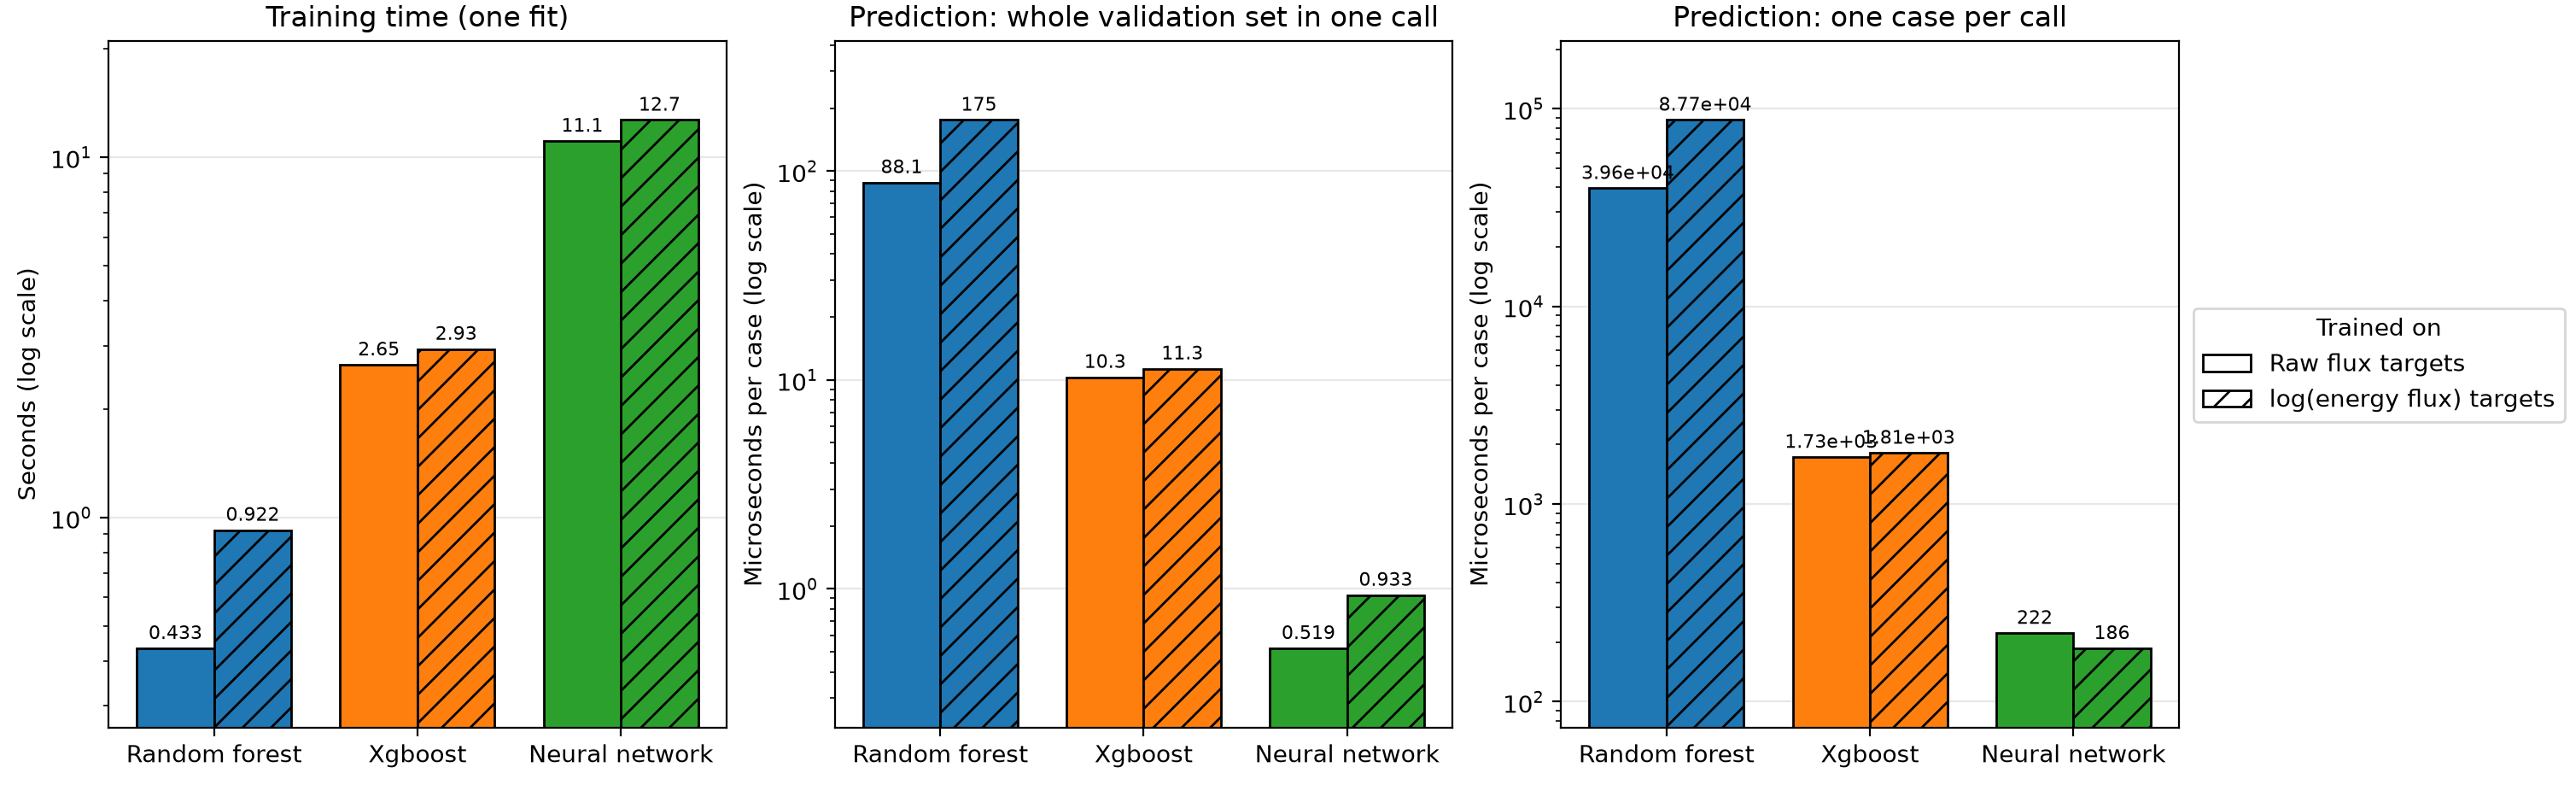
\includegraphics[width=\linewidth]{figures/scandb_timing.png}
  \caption{Training time (left) and prediction time per case (middle: whole
    validation set in one call; right: one case per call) for each model.
    Prediction times are medians over repeated calls. Hatched bars are models
    trained on log-transformed heat flux targets. Axes are logarithmic.}
  \label{fig:scandb-timing}
\end{figure}

\begin{figure}[htbp]
  \centering
  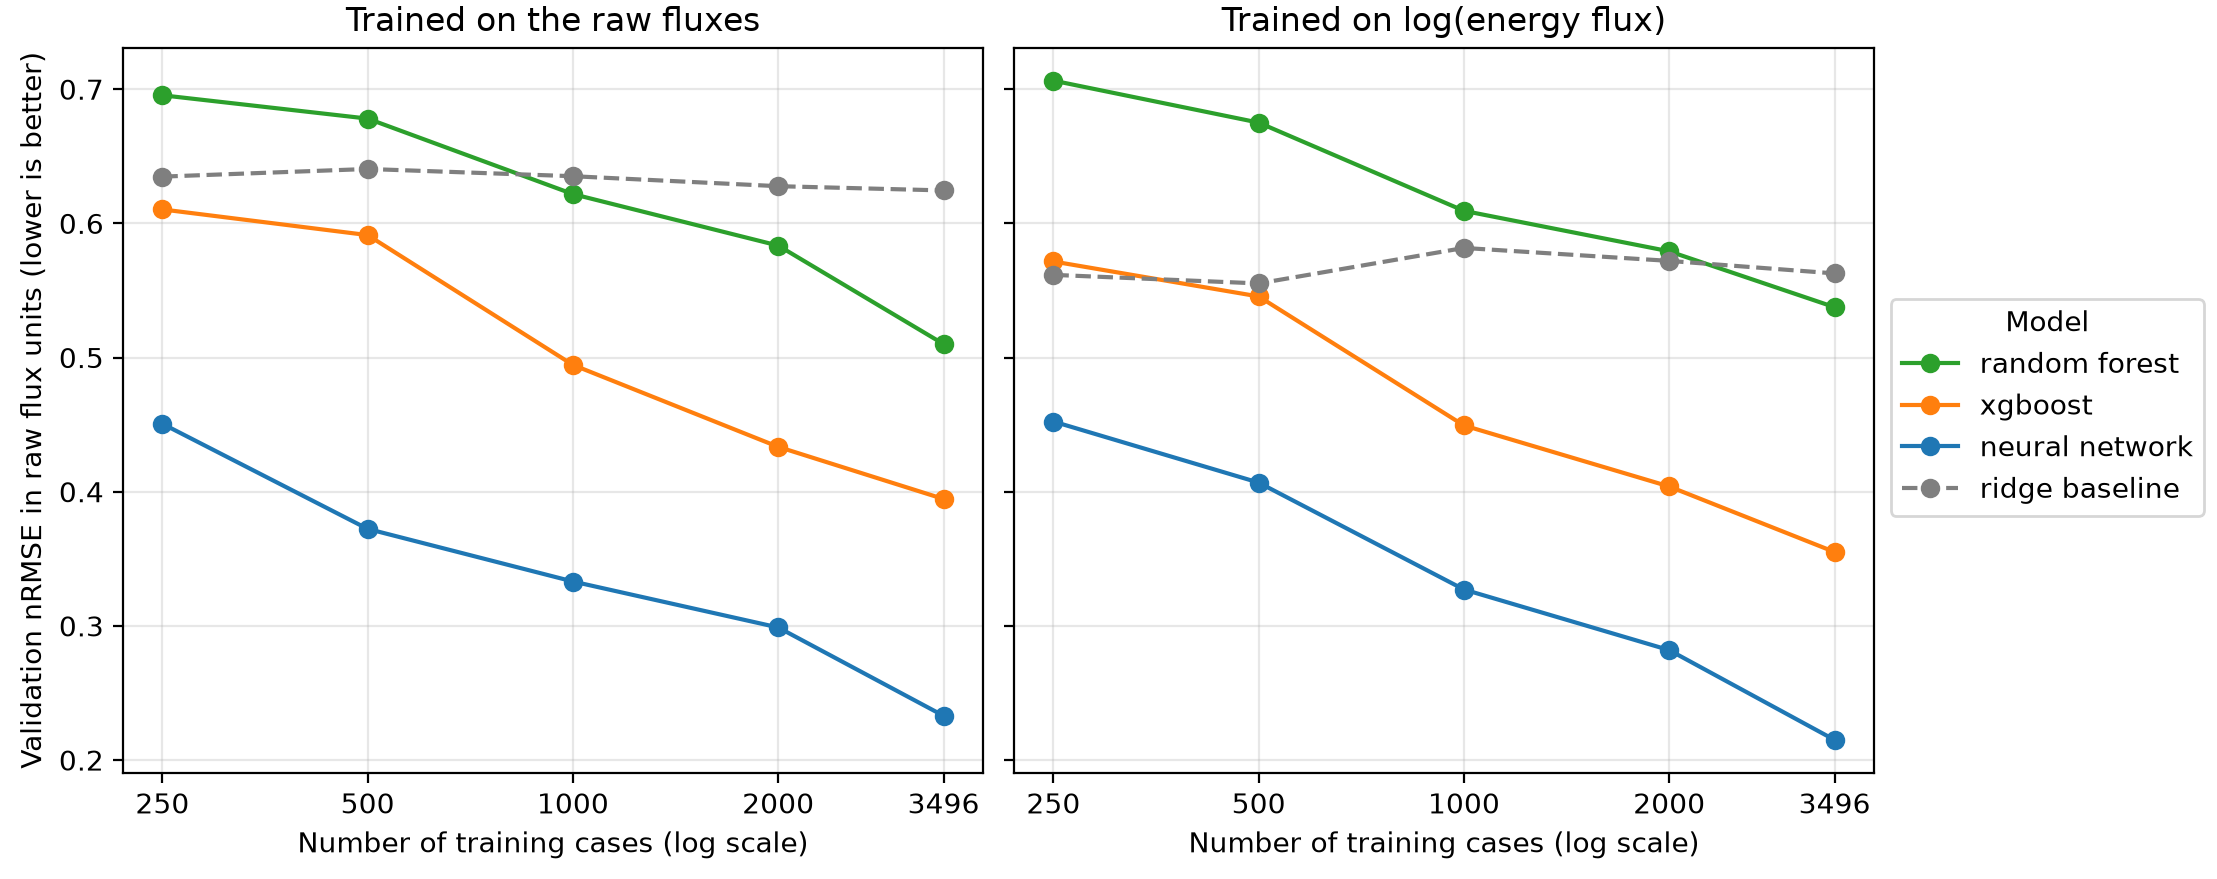
\includegraphics[width=\linewidth]{figures/scandb_learning_curves.png}
  \caption{Validation nRMSE against training set size for each model at its
    tuned hyperparameters. Left: models trained on raw fluxes. Right: models
    trained on log-transformed heat fluxes. The dashed line is the ridge
    baseline.}
  \label{fig:scandb-learning}
\end{figure}

\begin{figure}[htbp]
  \centering
  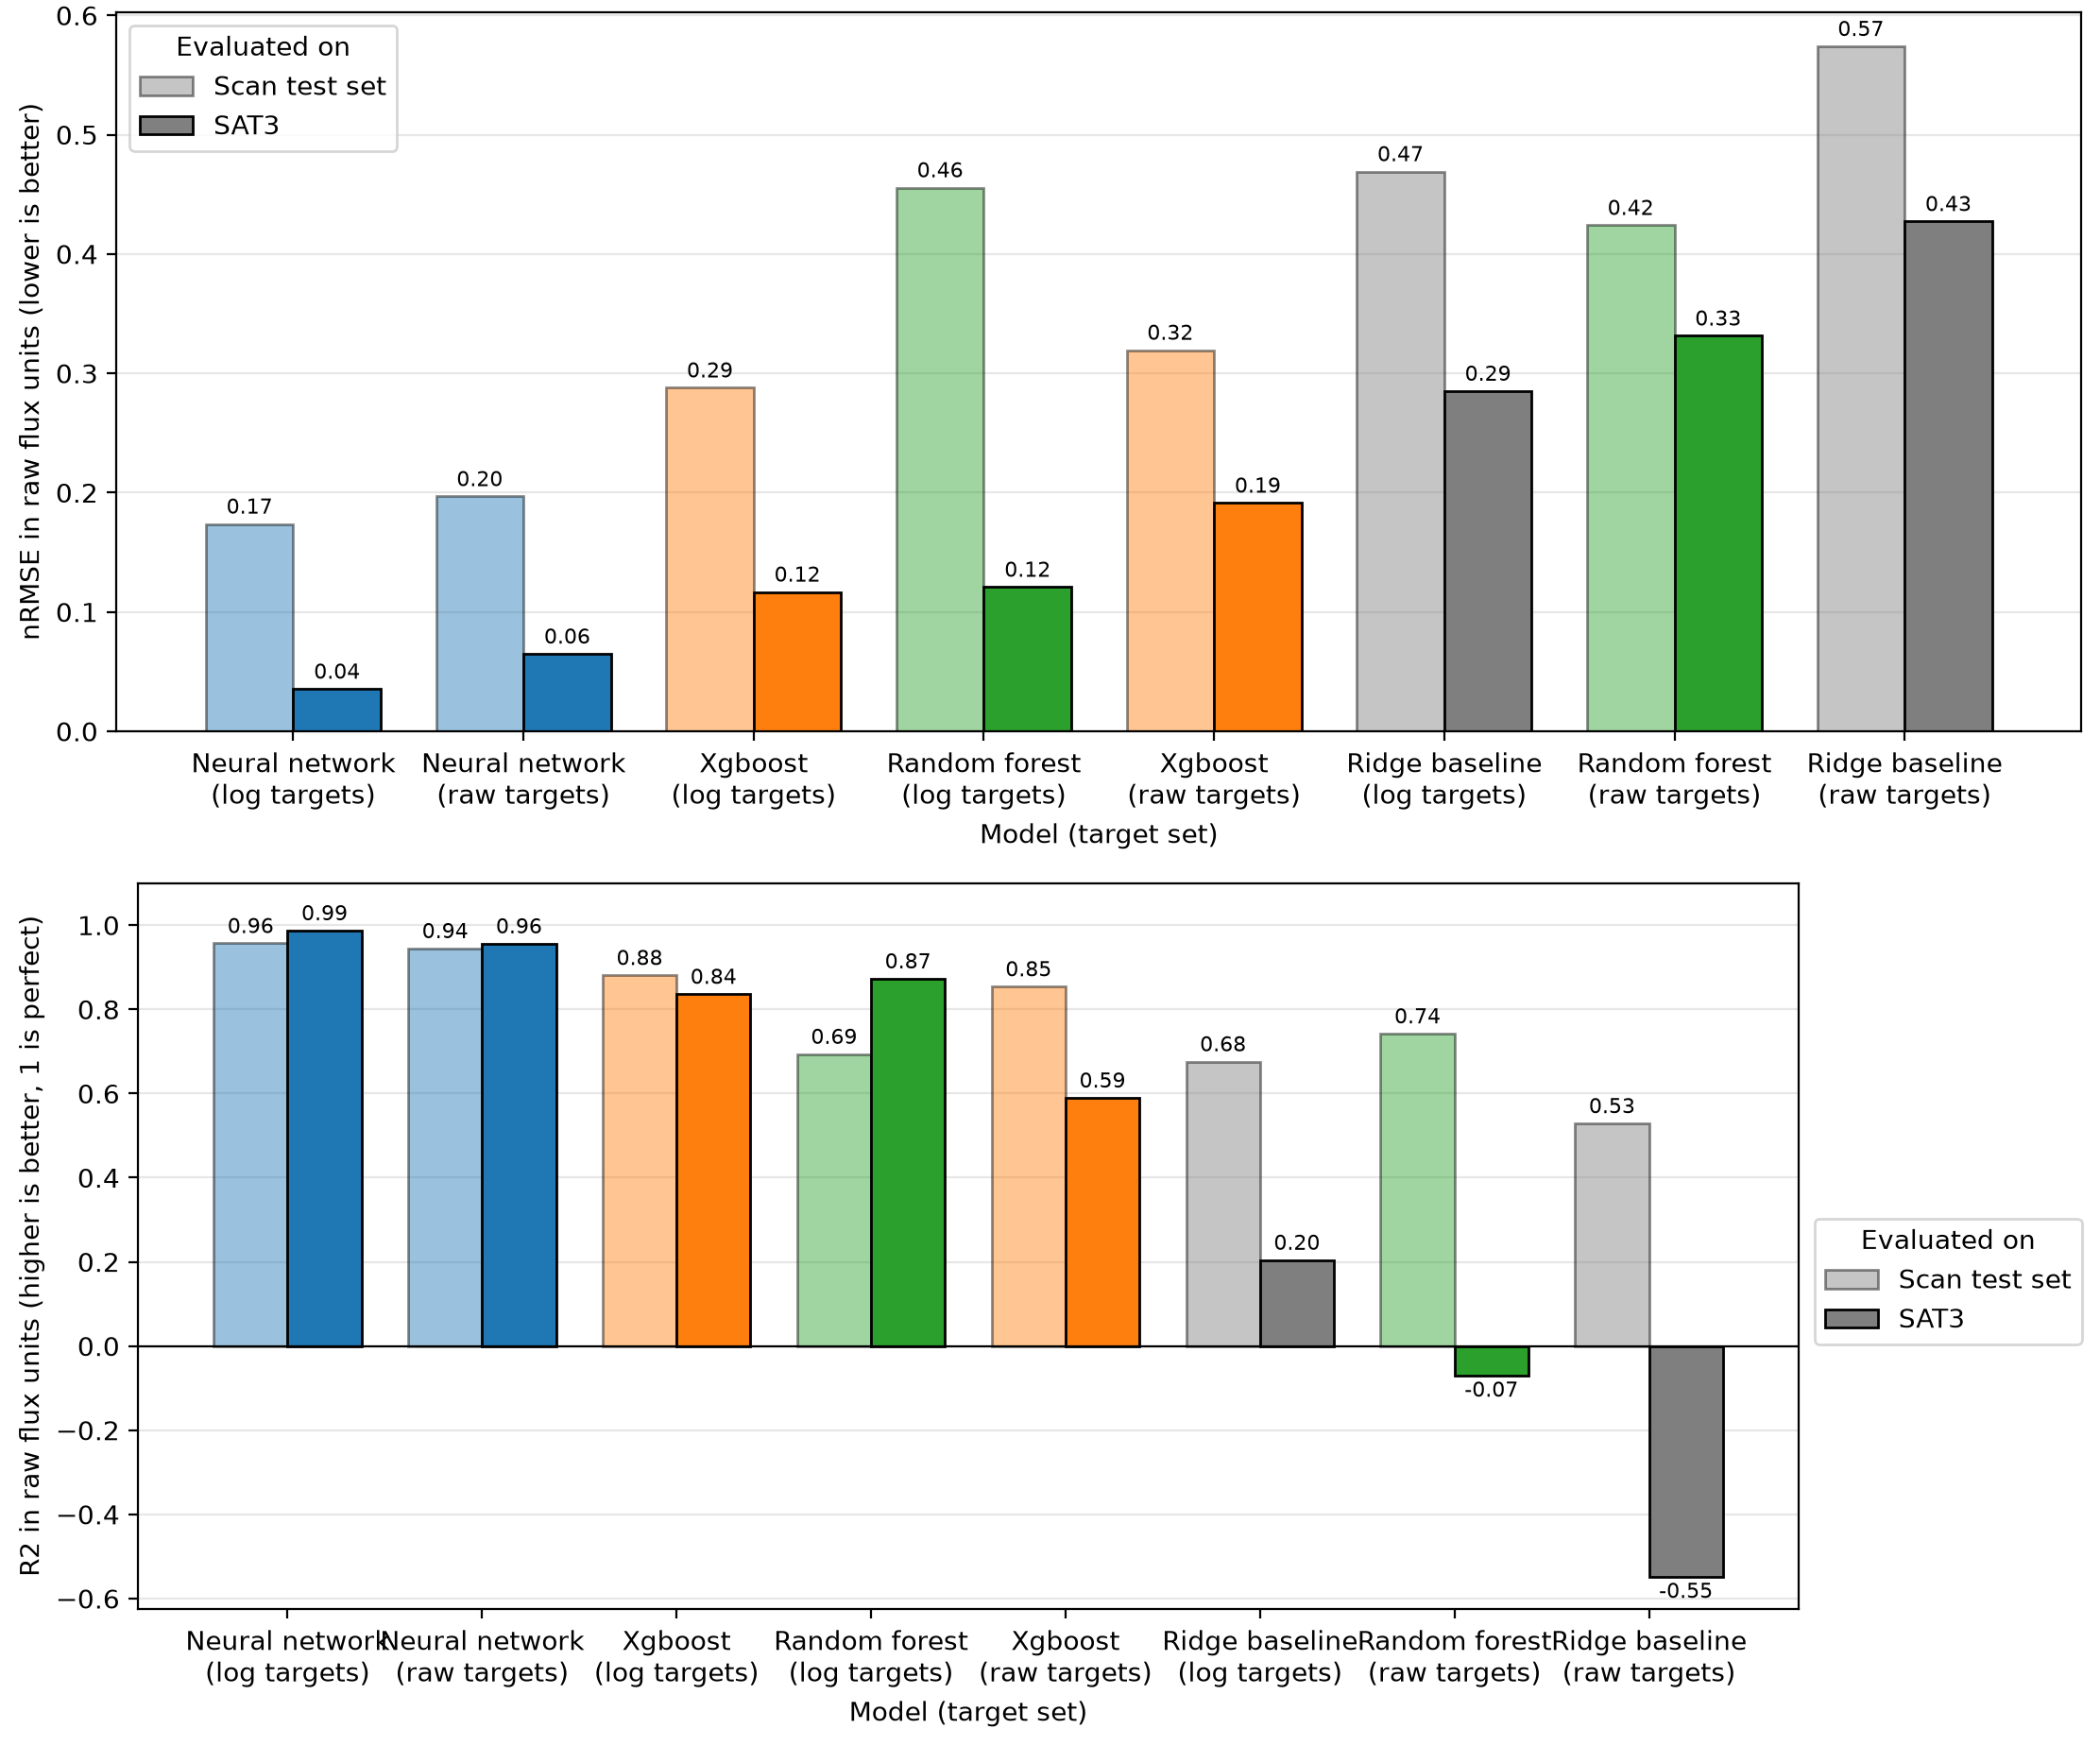
\includegraphics[width=0.85\linewidth]{figures/scandb_sat3_transfer.png}
  \caption{nRMSE (top) and $R^2$ (bottom) on the \texttt{scan\_db} test set
    (faded bars) and on the 43 SAT3 cases (solid bars) for each model and
    target set. Models were trained on \texttt{scan\_db} only, and nothing was
    refit for SAT3. $R^2$ below zero means worse than predicting the mean.}
  \label{fig:scandb-sat3}
\end{figure}

\subsection{Ensemble Accuracy Against Baselines and Activation Choice}
\label{sec:ensemble-results}

On the larger database, the accuracy ensemble outperformed the mean and
linear baselines on all three outputs (Table~\ref{tab:test}; setup in Section~\ref{sec:ensemble-methods}). Relative to
linear regression, test RMSE decreased by 59.6\% for ion heat, 61.8\% for
electron heat, and 77.2\% for particle flux. This does not establish
superiority over tree models evaluated elsewhere, or isolate the benefit of
averaging compared with an otherwise matched single network.

\begin{table}[htbp]
  \centering
  \caption{Performance on the same 750 random test cases from
    \texttt{scan\_db}. RMSE is in gyro-Bohm units. The test set was previously
    inspected; these are exploratory results for the selected GELU/ReLU model.}
  \label{tab:test}
  \small
  \setlength{\tabcolsep}{5pt}
  \begin{tabular}{lrrrrrr}
    \toprule
                          & \multicolumn{3}{c}{RMSE} & \multicolumn{3}{c}{$R^2$}                                                 \\
    \cmidrule(lr){2-4}\cmidrule(lr){5-7}
    Model                 & $Q_i$                    & $Q_e$                     & $\Gamma_e$ & $Q_i$    & $Q_e$    & $\Gamma_e$ \\
    \midrule
    Mean                  & 76.53                    & 60.20                     & 20.93      & $-0.009$ & $-0.010$ & $-0.011$   \\
    Linear                & 38.43                    & 29.48                     & 14.43      & 0.746    & 0.758    & 0.519      \\
    Five-network ensemble & 15.53                    & 11.27                     & 3.29       & 0.959    & 0.965    & 0.975      \\
    \bottomrule
  \end{tabular}
\end{table}

The controlled activation comparison selected GELU/ReLU, with a mean
normalized validation RMSE of 0.1806, compared with 0.1887 for GELU/tanh
(Table~\ref{tab:activations}). The 4.3\% aggregate improvement came from
ion heat and particle flux; electron-heat error increased. Replacing all
hidden activations with ReLU increased the aggregate error by 11.5\%
relative to GELU/tanh. Thus, neither a uniform activation replacement nor a
single aggregate score captures every target's response. These results
support the selected configuration under the fixed training setup, rather
than a universal ordering of activation functions.

\begin{table}[H]
  \centering
  \caption{Activation comparison on 750 validation cases. The first activation
    applies to both 64-unit layers and the second to the 8-unit layer.
    RMSE values are in gyro-Bohm units; $S$ is defined in Eq.~\ref{eq:selection}.}
  \label{tab:activations}
  \small
  \begin{tabular}{lrrrr}
    \toprule
    Activations & $S$    & $Q_i$ RMSE & $Q_e$ RMSE & $\Gamma_e$ RMSE \\
    \midrule
    GELU / ReLU & 0.1806 & 15.80      & 13.16      & 4.61            \\
    GELU / tanh & 0.1887 & 17.62      & 12.76      & 4.83            \\
    ReLU / tanh & 0.1935 & 18.15      & 12.93      & 4.99            \\
    ReLU / ReLU & 0.2105 & 18.67      & 15.62      & 5.19            \\
    \bottomrule
  \end{tabular}
\end{table}

\subsection{Learning Curves and Computational Cost}
\label{sec:learning-results}

The ensemble's errors decreased as the training set grew
(Figure~\ref{fig:learning}; protocol in Section~\ref{sec:eval-methods}). Mean normalized test RMSE decreased by 50.2\%
between 250 and 3,496 training cases, compared with 2.9\% for linear regression.
The ensemble improved by a further 11.1\% between 2,000 and 3,496 cases.
This run provides evidence that the model still benefited from additional
training examples over the tested range. It does not establish the amount
of data needed to reach a specified accuracy.

\begin{figure}[htbp]
  \centering
  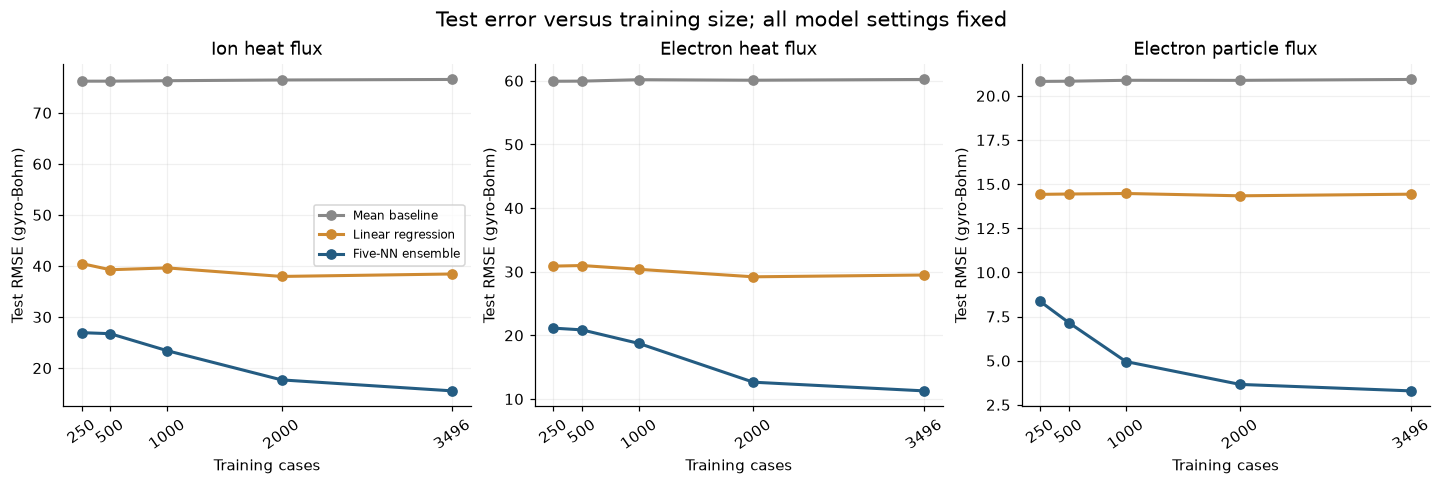
\includegraphics[width=\linewidth]{figures/learning_curves.png}
  \caption{Learning curves for the selected GELU/ReLU five-network
    ensemble and both baselines. Each point uses the same previously inspected
    750-case test set. Subsets form one nested sequence, with no resampling
    uncertainty bands. Settings are fixed, but larger subsets entail more
    minibatch updates per epoch.}
  \label{fig:learning}
\end{figure}

Training all five networks on a central processing unit (CPU) on UC San Diego's
Data Science/Machine Learning Platform (DSMLP) took 24.01\,s.
Median prediction latency was 0.814\,ms for one case, while a batch of 750
averaged 4.51\,$\mu$s per case. Training used four threads and prediction used
one. Prediction timings used seven repetitions after warmup and included
scaling, inverse transformations, and averaging, but excluded model loading,
file access, and feature construction. The supplied TGLF logs do not provide
elapsed runtimes, so these measurements do not support a measured
TGLF-to-surrogate speedup ratio.

\begin{samepage}
  \subsection{Starter-Set Trend and Sign Checks}
  \label{sec:trend-results}

  On the 43 starter cases, the selected ensemble achieved $R^2$ values of
  0.9702, 0.9973, and 0.9876 for $Q_i$, $Q_e$, and $\Gamma_e$, respectively.
  Nevertheless, it matched only 25 of 27 temperature-gradient directions and
  45 of 48 isotope directions, and predicted the wrong particle-flux sign in
  two cases. The validation-selected activation also improved starter-set
  $R^2$ for electron heat relative to GELU/tanh while reducing it for ion heat
  and particle flux. These checks show why an overall score should be read
  alongside local trends and failure cases.
\end{samepage}

\subsection{Gradient-Boosted Surrogate on \texttt{scan\_db}: Accuracy and Speed}
\label{sec:gbdt-results}

Table~\ref{tab:gbdt-test} reports the tuned \texttt{HistGradientBoostingRegressor}
surrogate from Section~\ref{sec:gbdt-methods} on its own 750-case
\texttt{scan\_db} test partition, alongside the mean and ridge baselines
fit on the same split. We report this as a separate table rather than adding
rows to Table~\ref{tab:starter} or Table~\ref{tab:test}: Table~\ref{tab:starter}
scores a different dataset (the 43 starter cases) and metric (letter-grouped
MAE), and Table~\ref{tab:test} is captioned as the same 750 test cases used to
select the five-network ensemble's activation function, whereas this
surrogate used its own independently drawn split of \texttt{scan\_db}, so its
750 test cases are not the same rows. The gradient-boosted surrogate reduced
test RMSE relative to its ridge baseline by 43.5\% for $Q_i$, 38.6\% for
$Q_e$, and 53.6\% for $\Gamma_e$, broadly consistent in direction with the
larger reductions reported for the five-network ensemble in
Section~\ref{sec:ensemble-results}, though the two are not evaluated on the
same split and should not be compared as if they were.

\begin{table}[htbp]
  \centering
  \small
  \setlength{\tabcolsep}{5pt}
  \begin{tabular}{lrrrrrr}
    \toprule
                   & \multicolumn{3}{c}{RMSE} & \multicolumn{3}{c}{$R^2$}                                                 \\
    \cmidrule(lr){2-4}\cmidrule(lr){5-7}
    Model          & $Q_i$                    & $Q_e$                     & $\Gamma_e$ & $Q_i$  & $Q_e$  & $\Gamma_e$ \\
    \midrule
    Mean           & 89.64                    & 62.41                     & 22.81      & $-0.000$ & $-0.002$ & $-0.002$ \\
    Ridge          & 62.31                    & 42.00                     & 15.74      & 0.517  & 0.546  & 0.523      \\
    GB surrogate   & 35.20                    & 25.80                     & 7.30       & 0.846  & 0.829  & 0.897      \\
    \bottomrule
  \end{tabular}
  \caption{Test-set performance of the tuned \texttt{HistGradientBoostingRegressor}
    surrogate (learning rate 0.08, 31 maximum leaf nodes, minimum leaf size
    10) and its baselines on 750 \texttt{scan\_db} test cases, a different
    split from Table~\ref{tab:test}. RMSE is in gyro-Bohm units.}
  \label{tab:gbdt-test}
\end{table}

Training each single-target model (300 boosting rounds with early stopping,
3,497 training cases) took 1.18\,s for $Q_i$, 1.69\,s for $Q_e$, and 1.26\,s
for $\Gamma_e$ on a single CPU core. Per-case prediction latency, measured by
repeating a 750-case batch call 100 times and dividing by the total number of
evaluations, was 12\,$\mu$s for $Q_i$, 15\,$\mu$s for $Q_e$, and 12\,$\mu$s for
$\Gamma_e$ --- roughly five orders of magnitude faster than the 3-second
per-case TGLF runtime assumed for this comparison, giving speedup factors of
about $2.4\times10^5$, $2.0\times10^5$, and $2.5\times10^5$, respectively.
These timings measure batched, amortized per-case cost rather than isolated
single-case calls, so they are not directly comparable to the single-call
latency reported for the five-network ensemble in
Section~\ref{sec:learning-results}.

\section{Uncertainty and Out-of-Range Results}
\label{sec:uncertainty-results}

This section evaluates the prediction intervals from the two methods in
Sections~\ref{sec:interval-methods} and~\ref{sec:disagreement-methods}, in the
same order. Sections~\ref{sec:coverage-results} to~\ref{sec:d3d-results}
report the quantile ensemble: its coverage, what its interval
width tracks, its behavior on inputs outside the training range, and the
DIII-D reference case. Section~\ref{sec:disagreement-results} reports the
15-network ensemble. All fluxes are in gyro-Bohm units, and all
comparisons are against TGLF, not experimental measurements.

\subsection{Interval Coverage and Calibration}
\label{sec:coverage-results}

Table~\ref{tab:coverage} gives the accuracy of the median prediction and the
coverage of the 5--95\% interval. On the test set the median reached $R^2$ of
0.876, 0.804, and 0.814 for $Q_i$, $Q_e$, and $\Gamma_e$, and coverage was
94.8\%, 93.9\%, and 98.0\%. Coverage is above the nominal 90\%, so the
intervals are somewhat conservative, most of all for particle flux. The
quantile intervals needed no separate calibration step.

\begin{table}[htbp]
  \centering
  \small
  \begin{tabular}{llrrr}
    \toprule
    Split      & Target     & $R^2$ (median) & nRMSE (median) & Coverage \\
    \midrule
    Validation & $Q_i$      & 0.879          & 0.347          & 0.956    \\
    Validation & $Q_e$      & 0.729          & 0.477          & 0.951    \\
    Validation & $\Gamma_e$ & 0.817          & 0.408          & 0.980    \\
    Test       & $Q_i$      & 0.876          & 0.304          & 0.948    \\
    Test       & $Q_e$      & 0.804          & 0.365          & 0.939    \\
    Test       & $\Gamma_e$ & 0.814          & 0.354          & 0.980    \\
    \bottomrule
  \end{tabular}
  \caption{Accuracy of the median and coverage of the 5--95\% interval for the
    quantile ensemble. Nominal coverage is 0.90. nRMSE is RMSE
    divided by the training-set standard deviation of that flux.}
  \label{tab:coverage}
\end{table}

Figure~\ref{fig:q-parity} shows the median and interval against the true flux
for 250 randomly chosen test cases. The widest intervals sit at the extremes of
the flux range, and most of the ion-heat misses are at low true flux. During
training, the mean interval width on the training set rose sharply after the
warmup epochs, peaked near epoch 50, and then fell while the loss kept
decreasing. It was still falling at epoch 150, so the interval widths depend on
how long the networks train.

\begin{figure}[htbp]
  \centering
  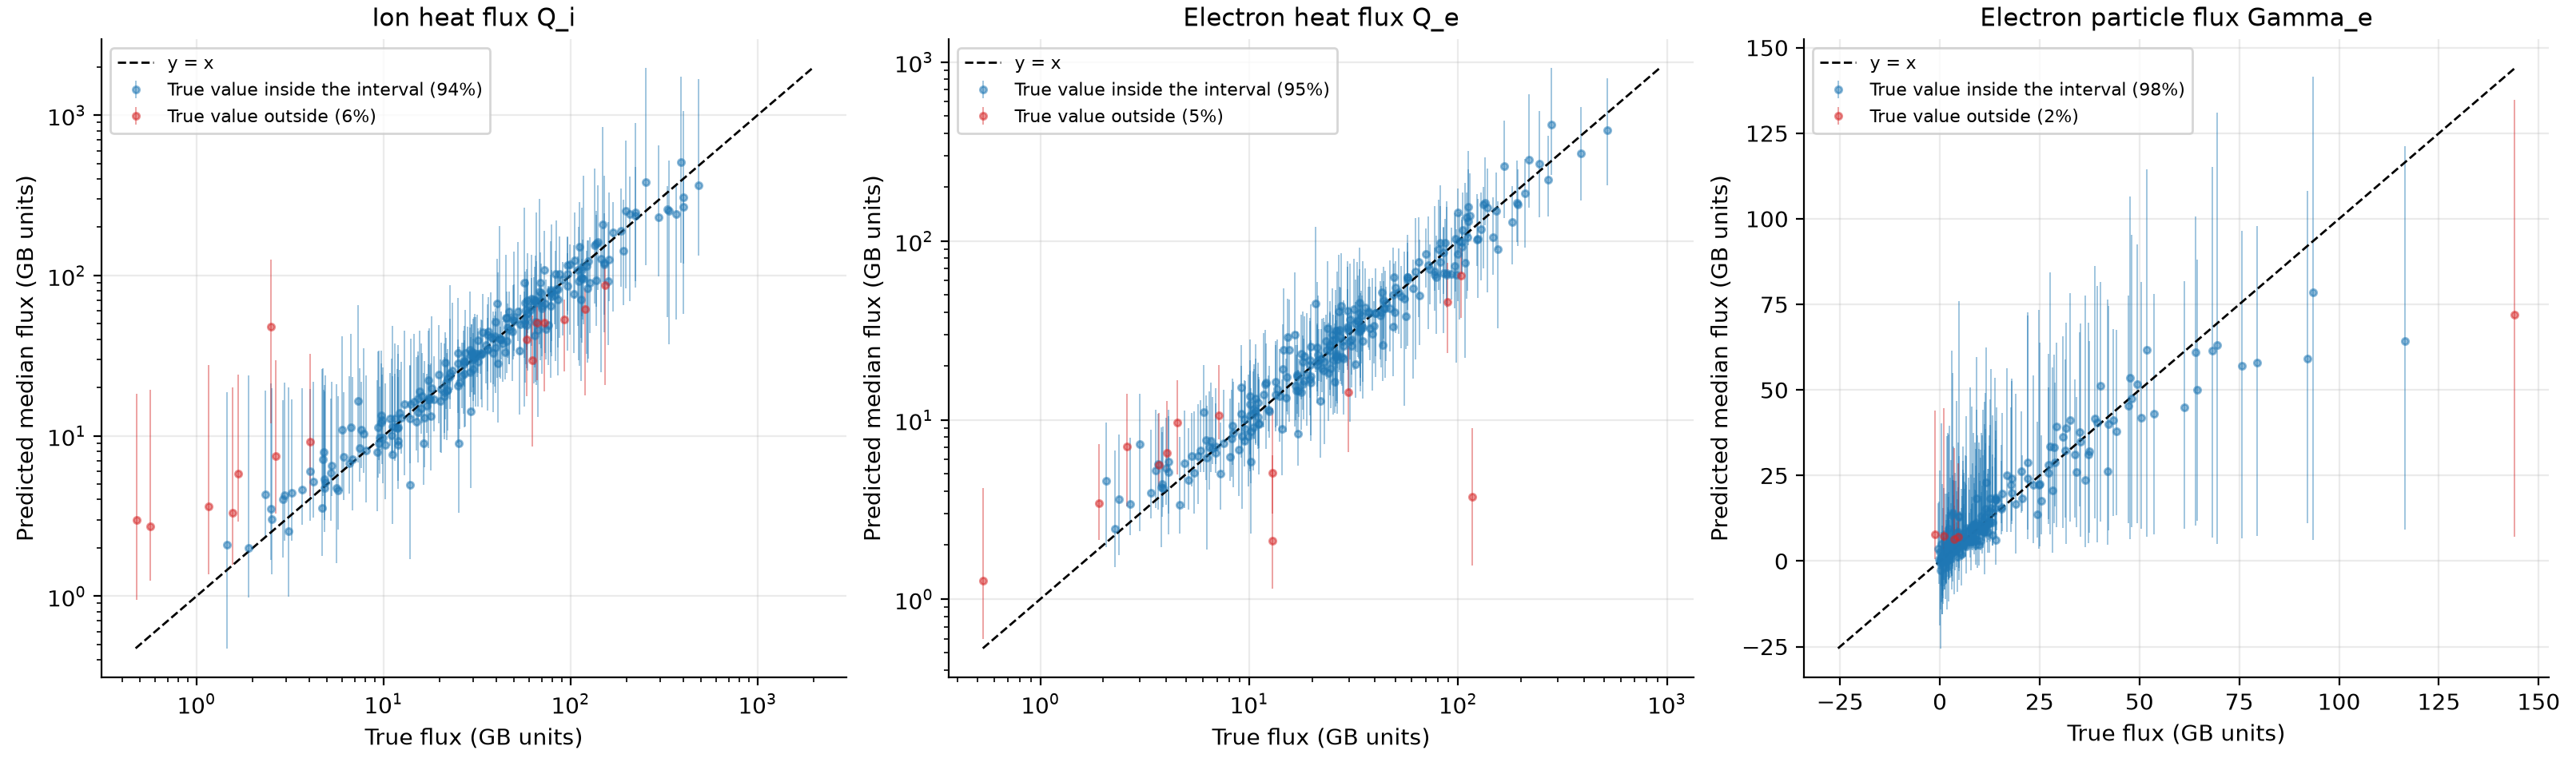
\includegraphics[width=\linewidth]{figures/q_parity_intervals.png}
  \caption{Predicted median and 5--95\% interval against the true flux for 250
    random test cases. Blue intervals contain the true value and red ones do
    not. The dashed line is $y = x$. Heat-flux axes are logarithmic.}
  \label{fig:q-parity}
\end{figure}

\subsection{Interval Width as an Error Indicator}
\label{sec:width-results}

Wider intervals go with larger errors (Figure~\ref{fig:q-error-width}). On the
test set the Spearman correlation between band width and absolute error is 0.46
for $Q_i$, 0.41 for $Q_e$, and 0.68 for $\Gamma_e$. The scatter is large, so
width is a rough warning and not a precise error estimate. For $\Gamma_e$,
width and error are both in raw units and both grow with the flux, so part of
its correlation is a scale effect.

\begin{figure}[htbp]
  \centering
  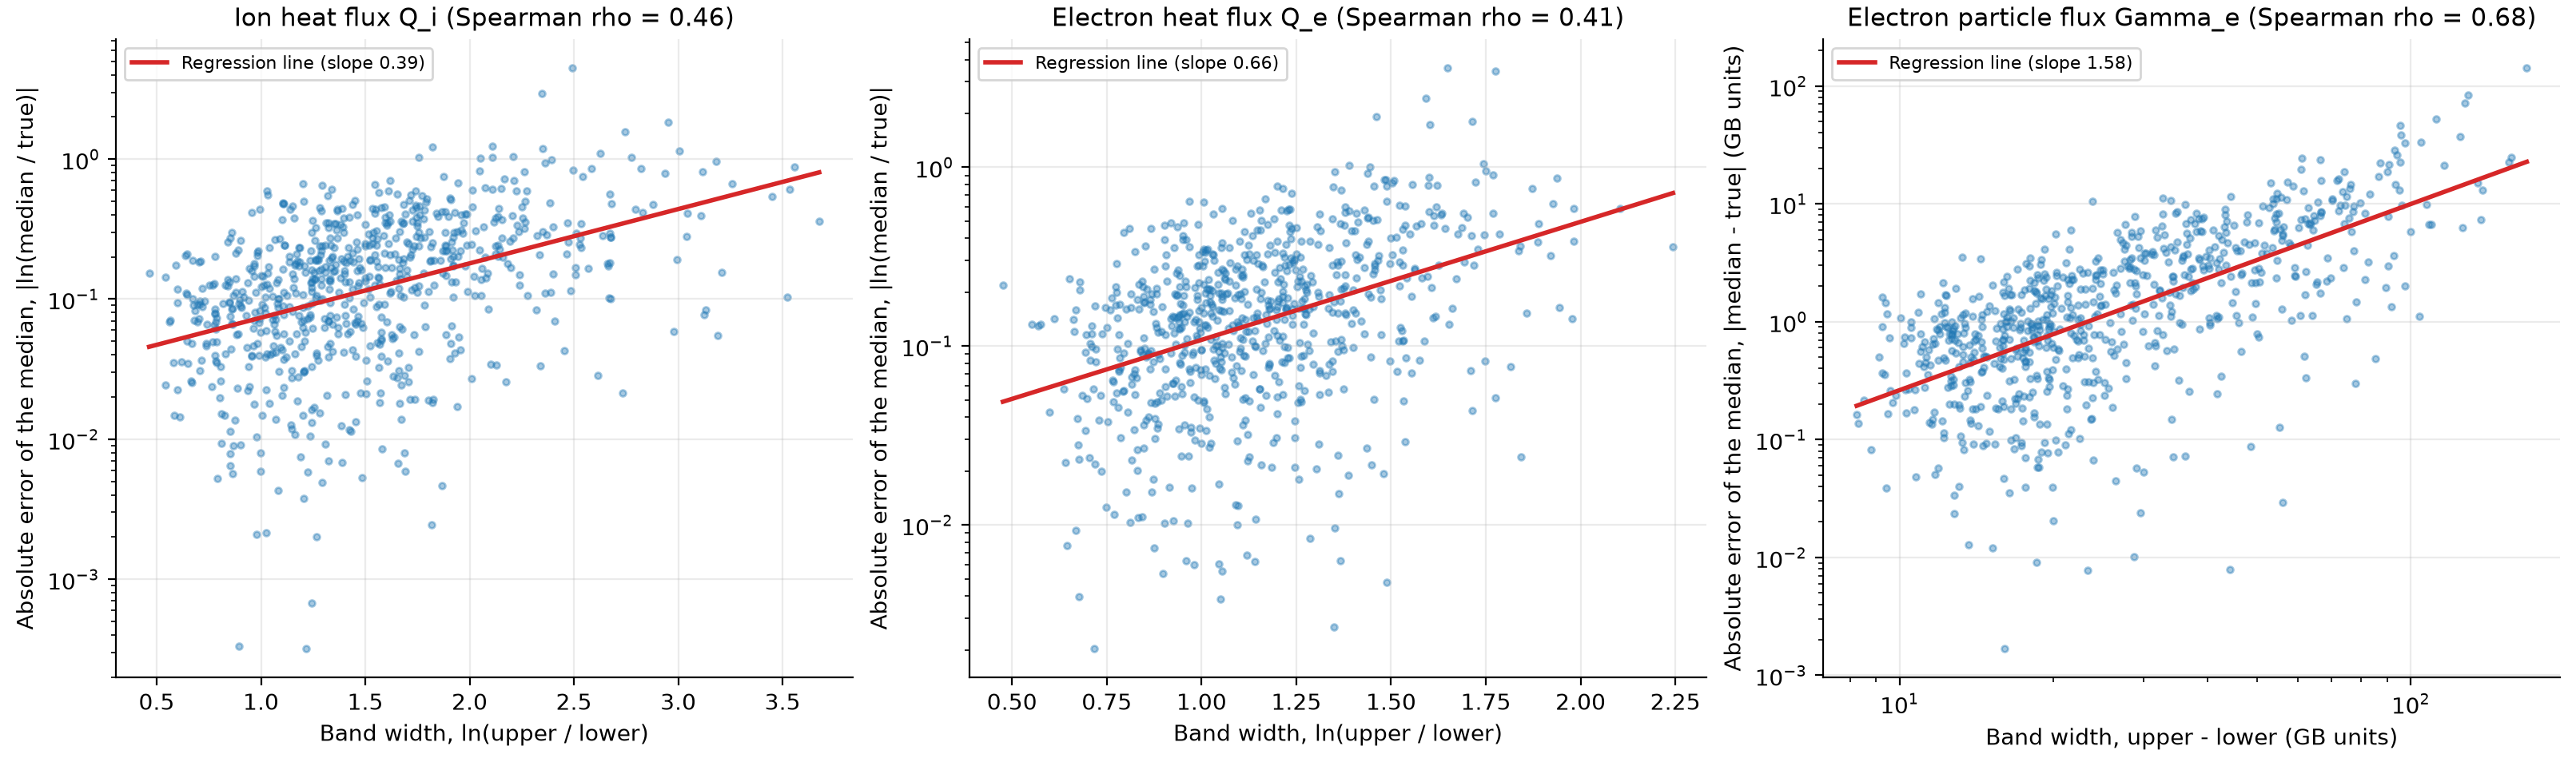
\includegraphics[width=\linewidth]{figures/q_error_vs_width.png}
  \caption{Absolute error of the median against band width on the test set. The
    red line is a least-squares fit of the logarithm of the error on the width.
    Both axes of the $\Gamma_e$ panel are in raw gyro-Bohm units.}
  \label{fig:q-error-width}
\end{figure}

Figure~\ref{fig:q-width-flux} shows how width depends on the true flux. For
$Q_i$ the pattern is a U: intervals are widest at very low flux (below about
3) and very high flux (above about 100), and narrowest between about 20 and 80.
These are also the flux ranges with the least training data, which is the main
evidence that interval width follows how much data the model has seen. For
$\Gamma_e$ the absolute width increases with flux, but this is mostly scale,
because the width stays in raw units. At very low flux the $\Gamma_e$ widths
also sit above their minimum, which is the other arm of the same U. $Q_e$ shows
only a weak relationship.

\begin{figure}[htbp]
  \centering
  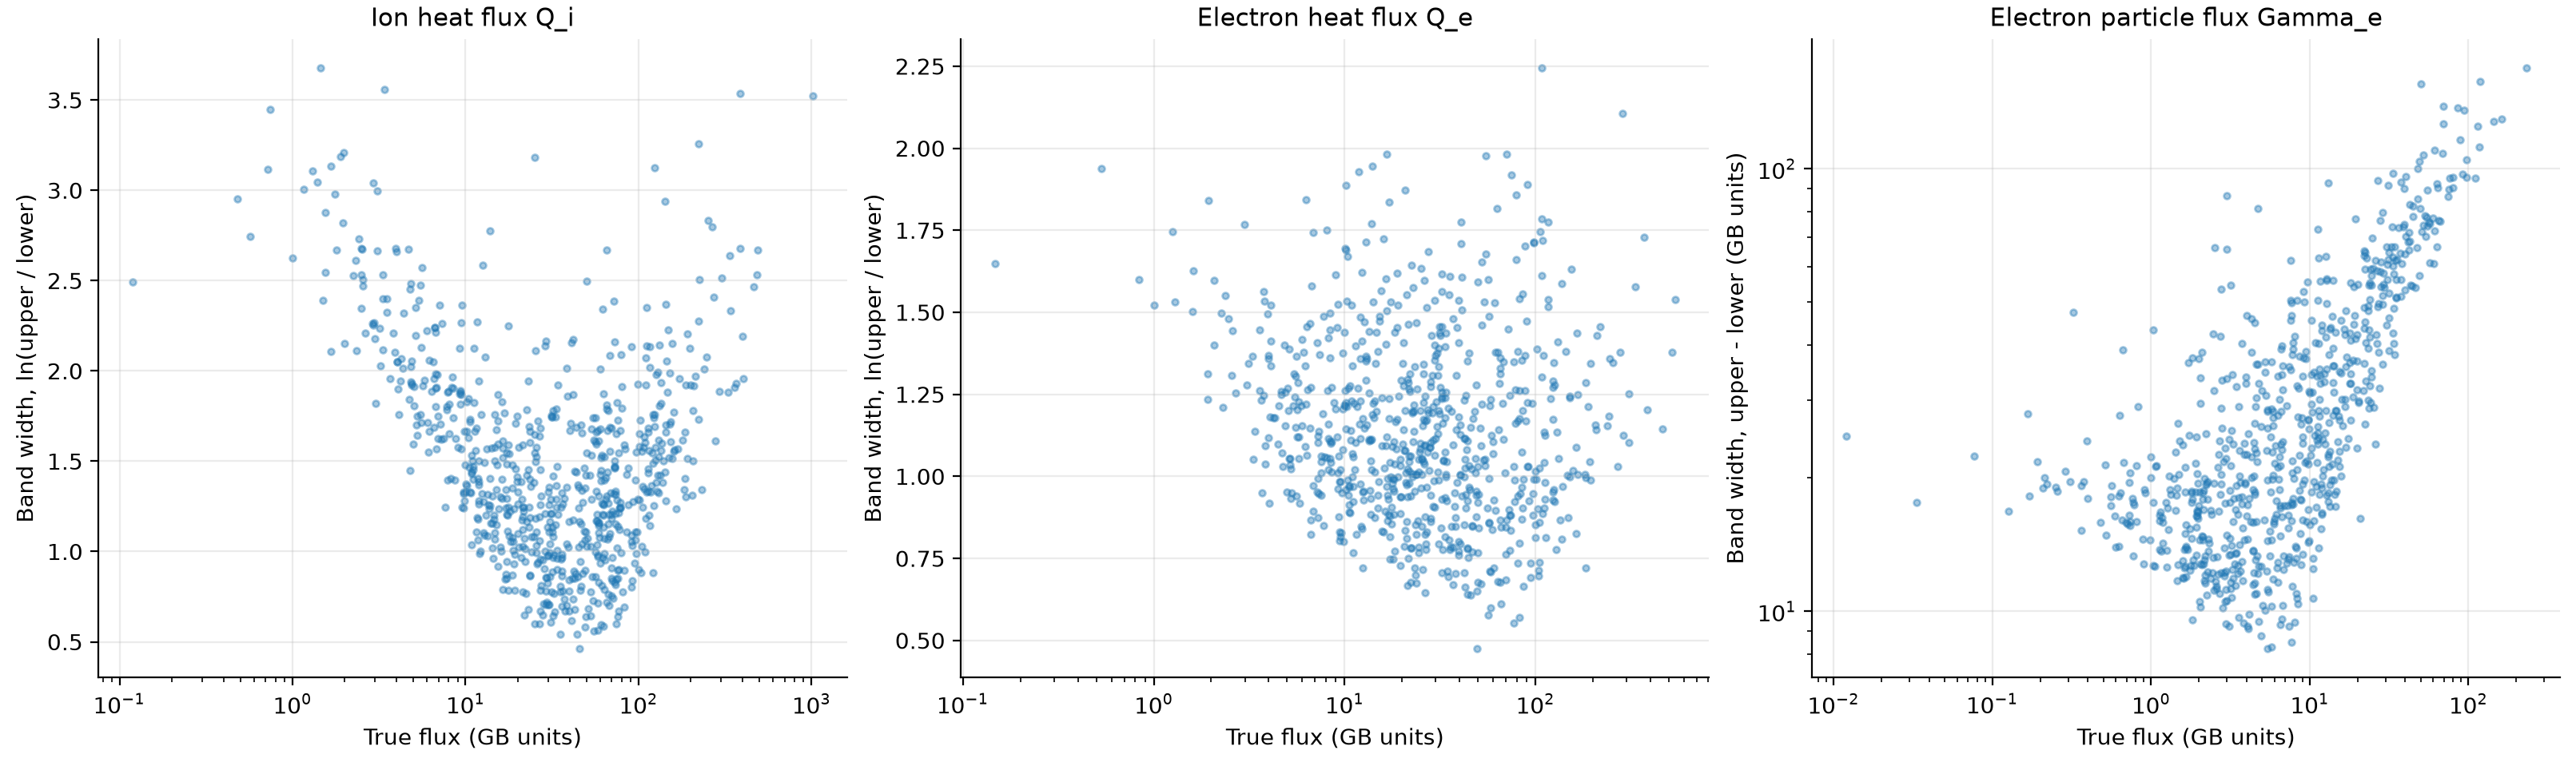
\includegraphics[width=\linewidth]{figures/q_width_vs_flux.png}
  \caption{Band width against the true flux on the test set. The heat-flux
    widths are $\ln(\text{upper}/\text{lower})$. The $\Gamma_e$ width is
    upper $-$ lower in gyro-Bohm units, so it grows with the flux.}
  \label{fig:q-width-flux}
\end{figure}

Figure~\ref{fig:q-width-training} tests the data-density explanation directly.
We cut each flux range into bins and counted the training cases in each bin.
Average relative width fell as the bin contained more training cases, with
Spearman correlations of $-0.97$ for $Q_i$ and $-0.78$ for $Q_e$. For
$\Gamma_e$ the per-bin correlation is only $-0.03$, although the average over
the third of bins with the fewest cases (about 17) is far above the third with
the most (about 3). A few bins with a median near zero inflate the relative
width there. This shows where the intervals are wide, but not whether the
network has learned the underlying physics.

\begin{figure}[htbp]
  \centering
  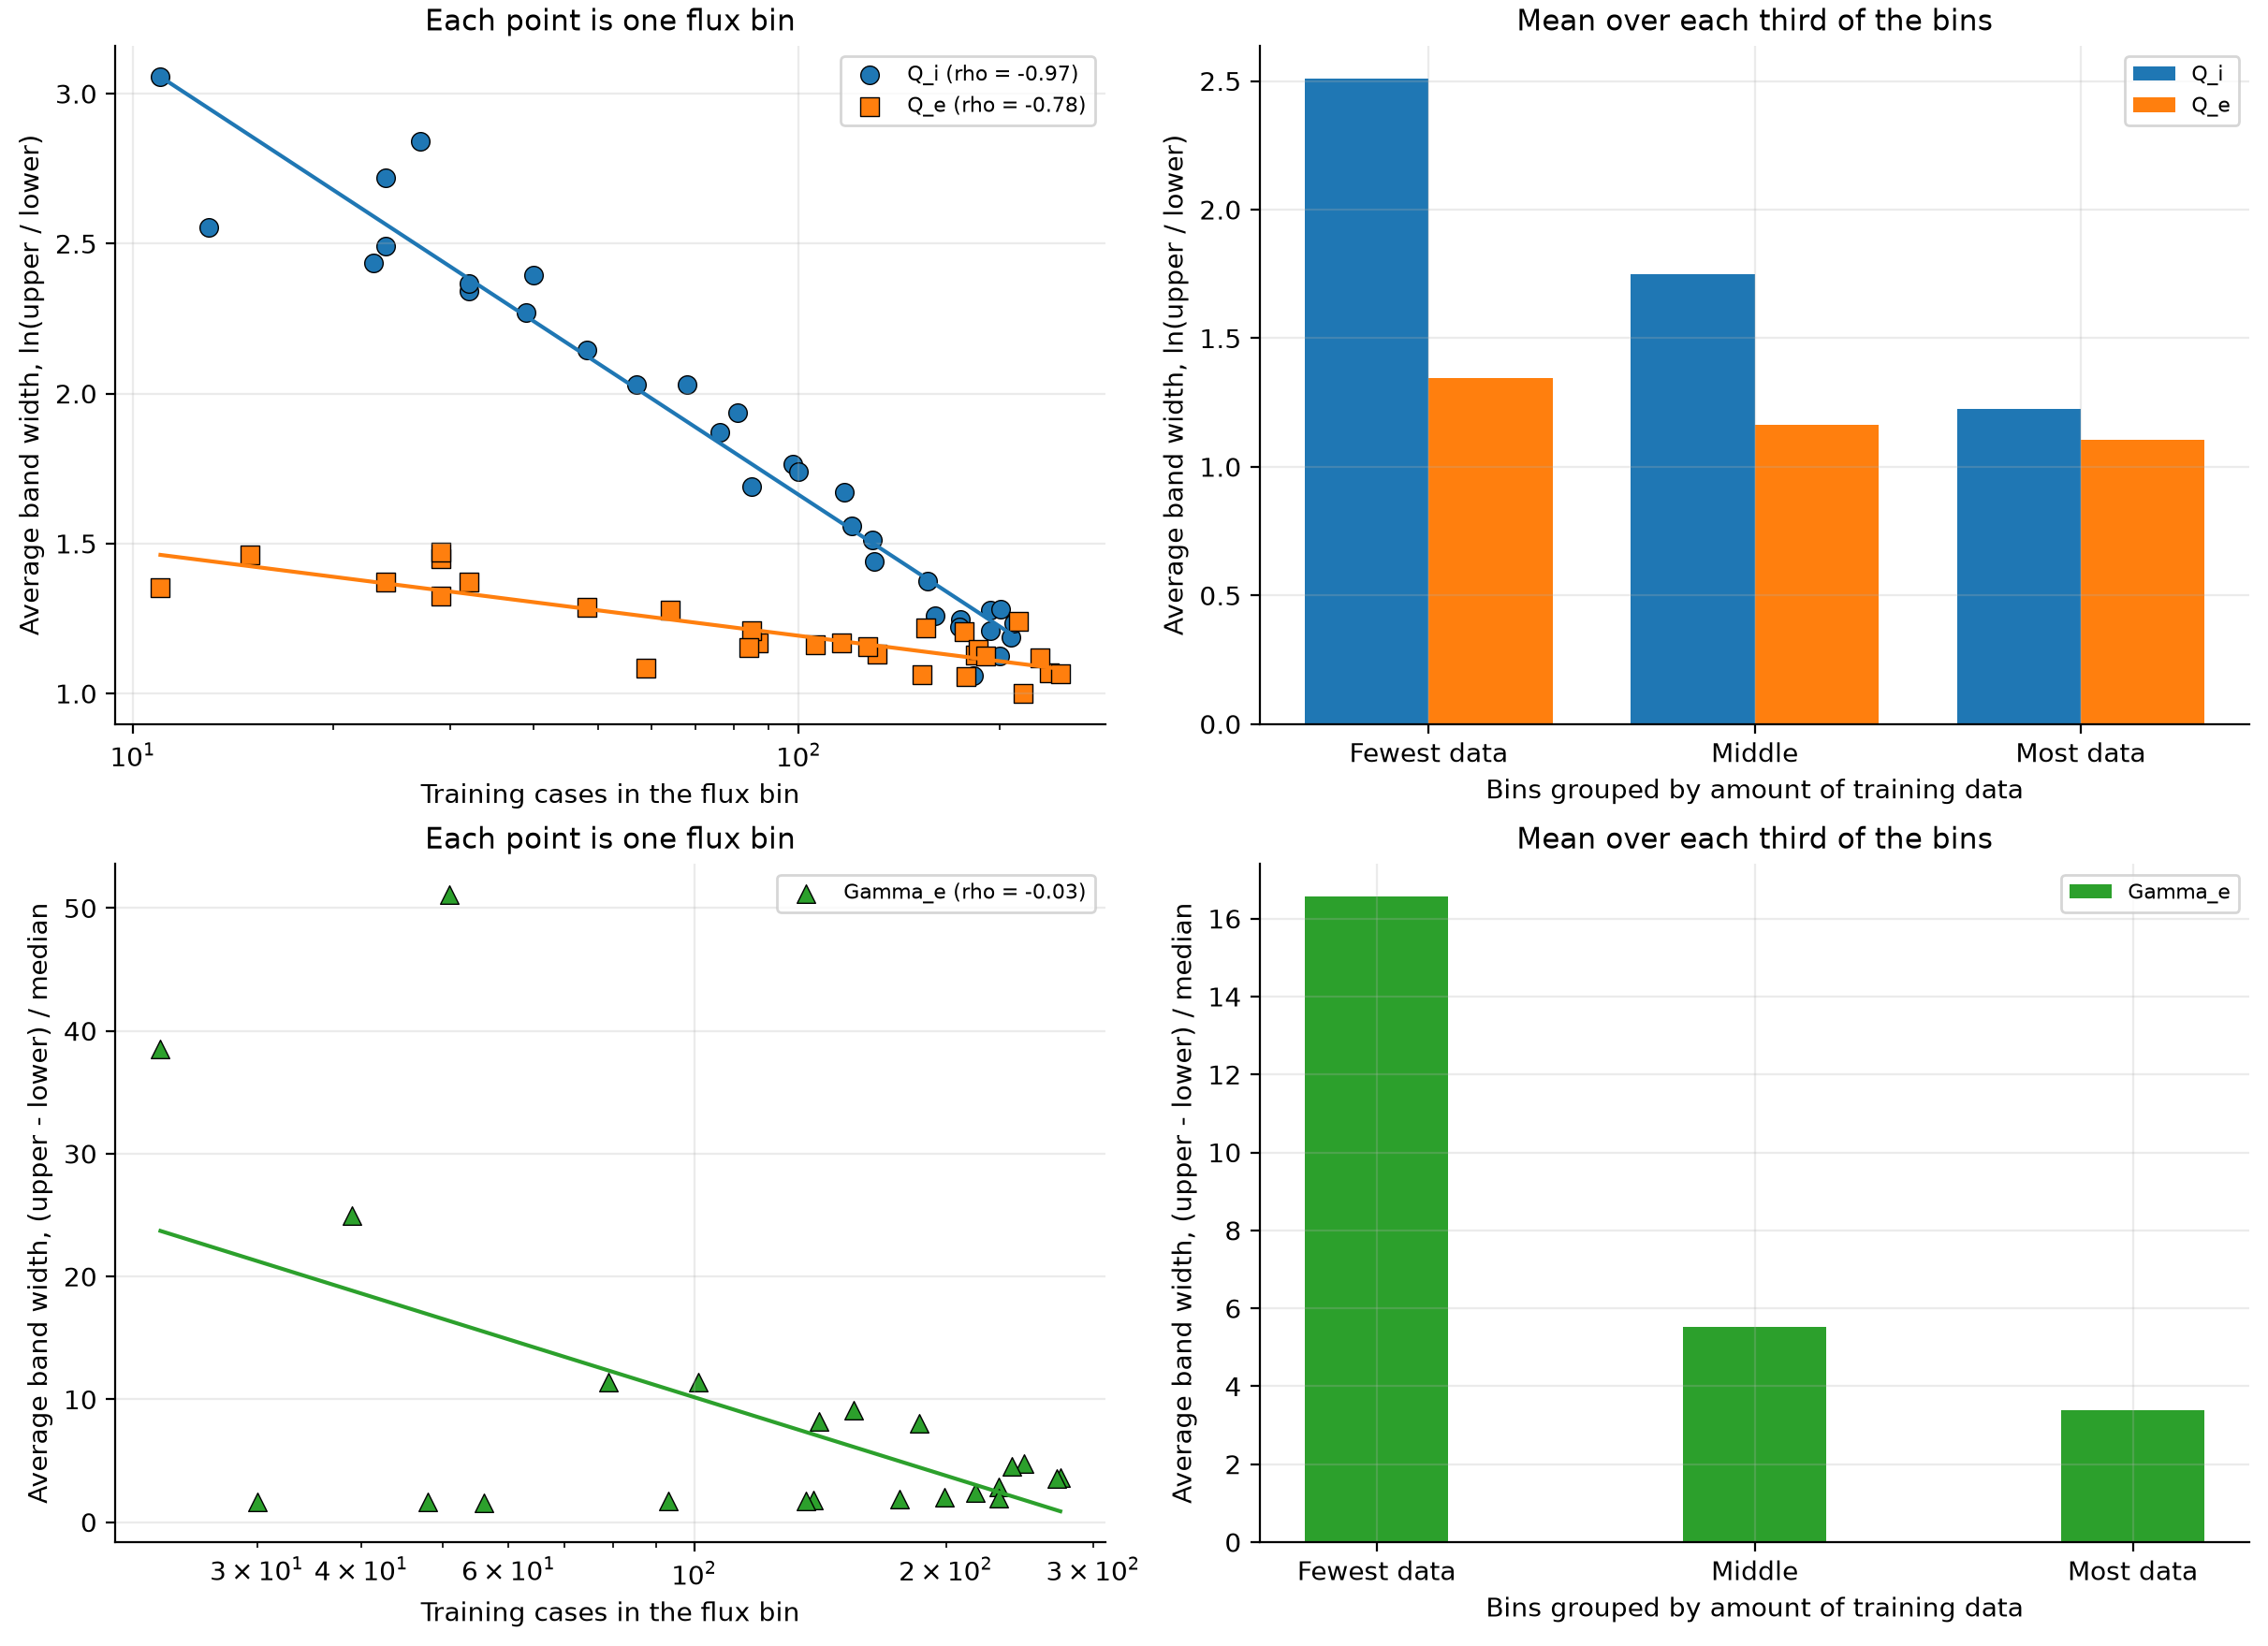
\includegraphics[width=0.8\linewidth]{figures/q_width_vs_training.png}
  \caption{Average relative band width against the number of training cases in
    the flux bin (left) and averaged over the third of bins with the fewest,
    middle, and most training cases (right), on the test set. The top row shows
    the heat fluxes and the bottom row shows $\Gamma_e$.}
  \label{fig:q-width-training}
\end{figure}

The inputs most correlated with relative width differ by flux. For $\Gamma_e$ it
is the density gradient \texttt{RLNS\_1} (Spearman $-0.69$ on the test set,
so smaller gradients give wider intervals), followed by log collision
frequency ($0.35$). For $Q_e$ it is \texttt{RLNS\_1} ($-0.45$) and
\texttt{RLTS\_1} ($0.28$). For $Q_i$ the correlations are all small: elongation
(0.26), \texttt{RLTS\_2} ($-0.27$), and \texttt{TAUS\_2} ($-0.25$). Inputs also
move the flux itself, so part of this reflects flux level, most of all for
$\Gamma_e$, whose relative width is inflated where the median is near zero.

\subsection{Behavior on Out-of-Range Inputs}

Error was higher on the outside-range groups than on the ordinary test set in
22 of the 27 group and flux combinations, and up to about ten times higher for
$Q_e$ when \texttt{RLNS\_1} is pushed out of range (Figure~\ref{fig:q-ood}).
Coverage on these groups stayed between 0.80 and 1.00, with 30 cases per
group.

\begin{figure}[htbp]
  \centering
  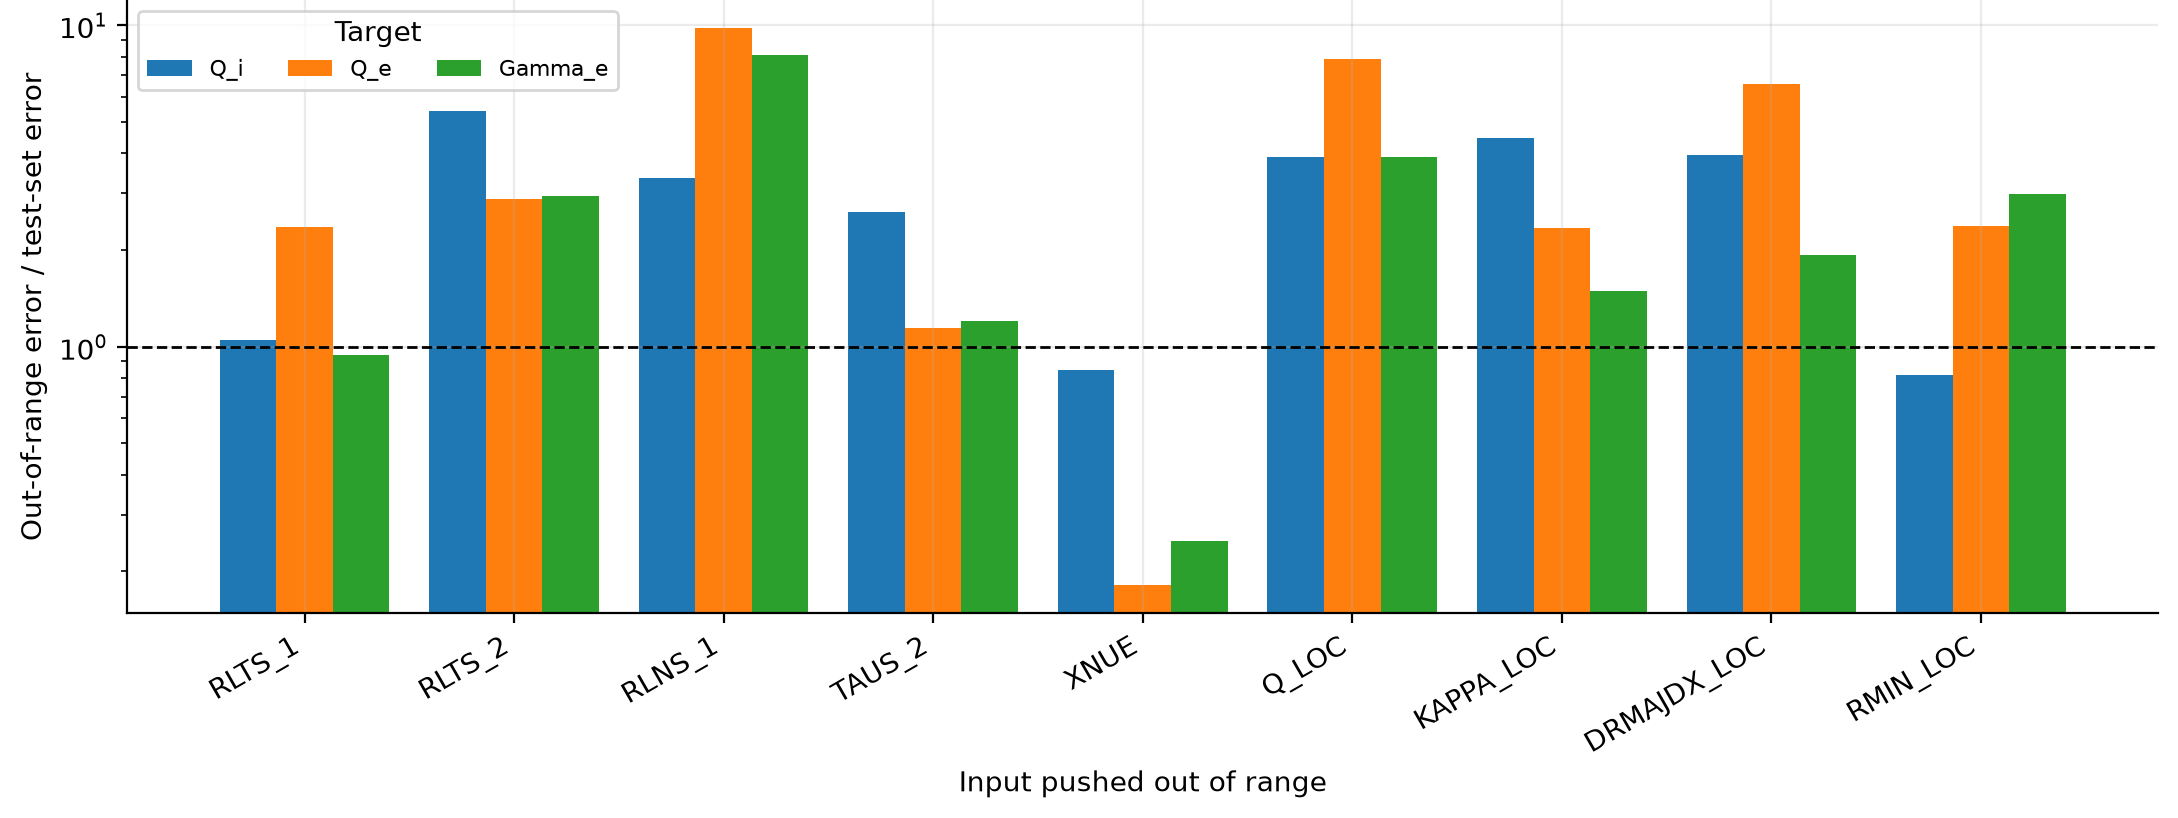
\includegraphics[width=0.85\linewidth]{figures/q_ood_error_ratio.png}
  \caption{nRMSE of the median on each outside-range group divided by the
    nRMSE on the in-range test set. The dashed line at 1 marks equal error.
    The vertical axis is logarithmic, and each group has 30 cases.}
  \label{fig:q-ood}
\end{figure}

Interval width followed this only partly. For $Q_i$ and $Q_e$, width rose with
distance beyond the scan range for most inputs (Spearman 0.05 to 0.67, largest
for \texttt{Q\_LOC} and \texttt{XNUE}). For $\Gamma_e$ the correlation was
near zero for most inputs. There are also direct counterexamples. For
\texttt{RLNS\_1}, the $Q_e$ nRMSE was 3.59 (against 0.37 in range) and $R^2$ was
$-0.52$, yet the median relative width was 1.03, slightly below the in-range
1.11. The \texttt{XNUE} group went the other way: its nRMSE was lower than
in range, but $R^2$ was lower for all three fluxes (0.51, 0.58, and 0.28
against 0.88, 0.80, and 0.81) and the intervals were wider, for example a
median $\Gamma_e$ relative width of 7.8 against 3.0. A wide interval is
therefore a useful warning for most outside-range inputs, but a narrow one does
not guarantee accuracy.

\subsection{DIII-D Input-Uncertainty Case Study}
\label{sec:d3d-results}

DIII-D is a tokamak at General Atomics, and $r/a$ is the position inside the
plasma as a fraction of its minor radius, where 0 is the center and 1 is the
edge. The reference case is one real DIII-D plasma at $r/a = 0.5$, halfway
out, expressed as a set of TGLF inputs in the \texttt{scan\_db} format (the
gradients, collision frequency, safety factor, and so on, with all other TGLF
settings as in \texttt{scan\_db}). At these inputs TGLF gives $Q_i = 4.31$,
$Q_e = 3.63$, and $\Gamma_e = 0.387$.

Measured plasma profiles are not exact, so each uncertain input carries an
error bar: $\pm 10\%$ for the temperature and density gradients, the
temperature ratio, and the safety-factor gradient, $\pm 20\%$ for collision
frequency, and $\pm 5\%$ for the safety factor. The elongation, Shafranov
shift, minor radius, and ion mass are held fixed. This case study asks how much
those input errors move the predicted fluxes, and whether the surrogate
reproduces that spread. TGLF answers the first question by running 300 input
sets sampled within the bars. Input errors of 5--20\% spread the TGLF fluxes by
$\pm 42\%$, $\pm 45\%$, and $\pm 80\%$ of the mean for $Q_i$, $Q_e$, and
$\Gamma_e$, where each figure is half of the 5--95\% range as a percentage of
the mean. We answer the second question by passing 10,000 random input sets
from the same bars through the surrogate, which took 0.041\,s in total, and
keeping its median prediction. The 10,000 draws are inputs only and have no
TGLF counterparts.

Figure~\ref{fig:d3d-compare} shows that the surrogate sits above TGLF. The mean
surrogate flux was 5.50 against 4.44 for $Q_i$, 5.31 against 4.12 for $Q_e$,
and 1.38 against 0.48 for $\Gamma_e$. When the surrogate is run on the same 300
input sets as TGLF, the correlation with TGLF is high (0.95, 0.89, and 0.92),
so it responds to the inputs in the same direction, but its predictions are
above TGLF's on average by 22\%, 29\%, and a factor of 2.9. Its relative spread
(standard deviation over mean) is also smaller, 0.17, 0.14, and 0.26 against
0.25, 0.27, and 0.49. The surrogate is therefore biased upward and under-reacts
to the input uncertainty at this operating point.

\begin{figure}[htbp]
  \centering
  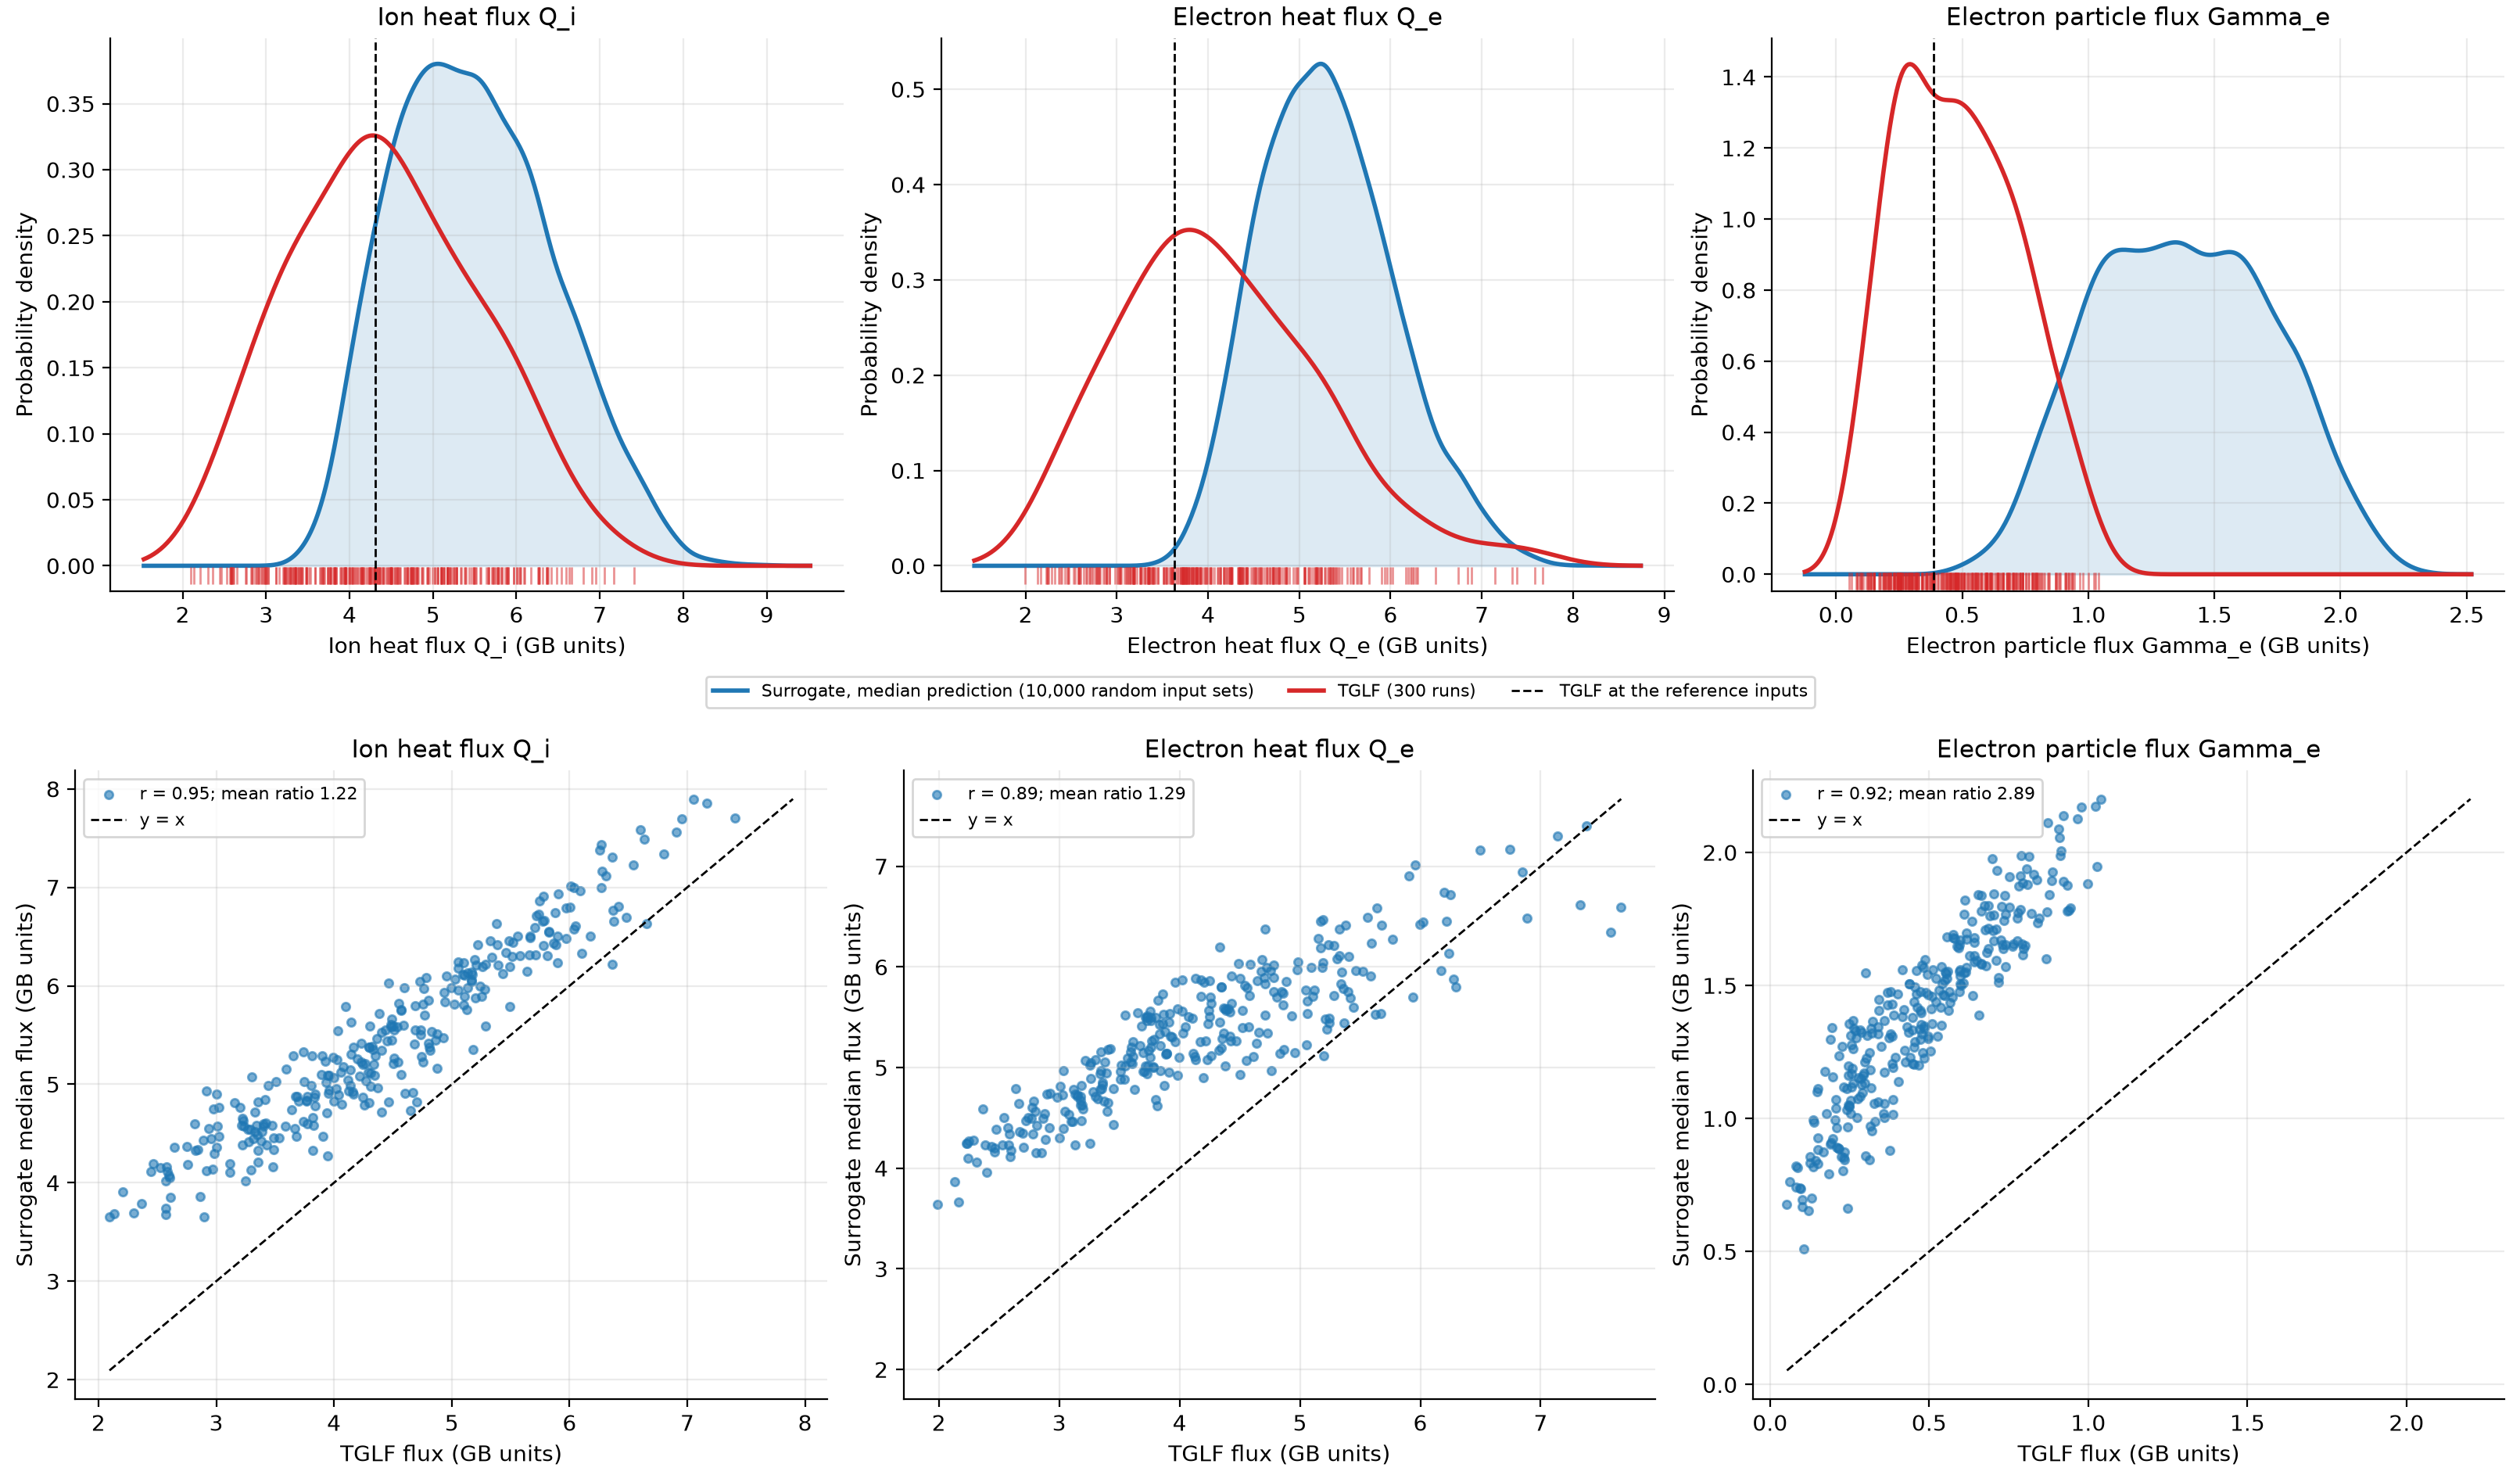
\includegraphics[width=\linewidth]{figures/d3d_surrogate_vs_tglf.png}
  \caption{Top: distribution of the flux under the input error bars for the
    surrogate (median prediction, 10,000 draws, blue) and TGLF (300 runs, red).
    The dashed line is TGLF at the reference inputs. Bottom: surrogate against
    TGLF on the same 300 input sets, with the line $y = x$. The legend gives
    the correlation and the mean ratio of surrogate to TGLF.}
  \label{fig:d3d-compare}
\end{figure}

The cause of this bias is not established, but the inputs give a hint. All 11
DIII-D inputs lie inside the training scan (Figure~\ref{fig:d3d-inputs}), but
four are in its lowest quarter: the density gradient \texttt{RLNS\_1} (8th
percentile), the magnetic shear (11th), \texttt{RLTS\_2} (22nd), and
\texttt{Q\_LOC} (23rd). The density gradient matters most for particle flux. It
is the input most strongly linked to wider $\Gamma_e$ intervals
(Section~\ref{sec:width-results}), so the DIII-D case sits where the model is
least certain about $\Gamma_e$.

To see why the surrogate reacts too little to the input errors, we changed one
input at a time within its error bar and measured how much the flux moved
(Table~\ref{tab:d3d-sensitivity}). The surrogate responds about half as
strongly as TGLF to the density gradient. Its flux moves by 14.0\% against
32.9\% for $Q_e$ and by 34.4\% against 68.0\% for $\Gamma_e$. With all inputs
varied together, the surrogate's spread is one half to two thirds of TGLF's.
TGLF was only run with all inputs varying together, so its per-input values
are estimated from a straight-line fit to the 300 runs, which explains 88\% to
91\% of the variation ($R^2$ of 0.91, 0.88, and 0.91). They are approximate.

\begin{figure}[htbp]
  \centering
  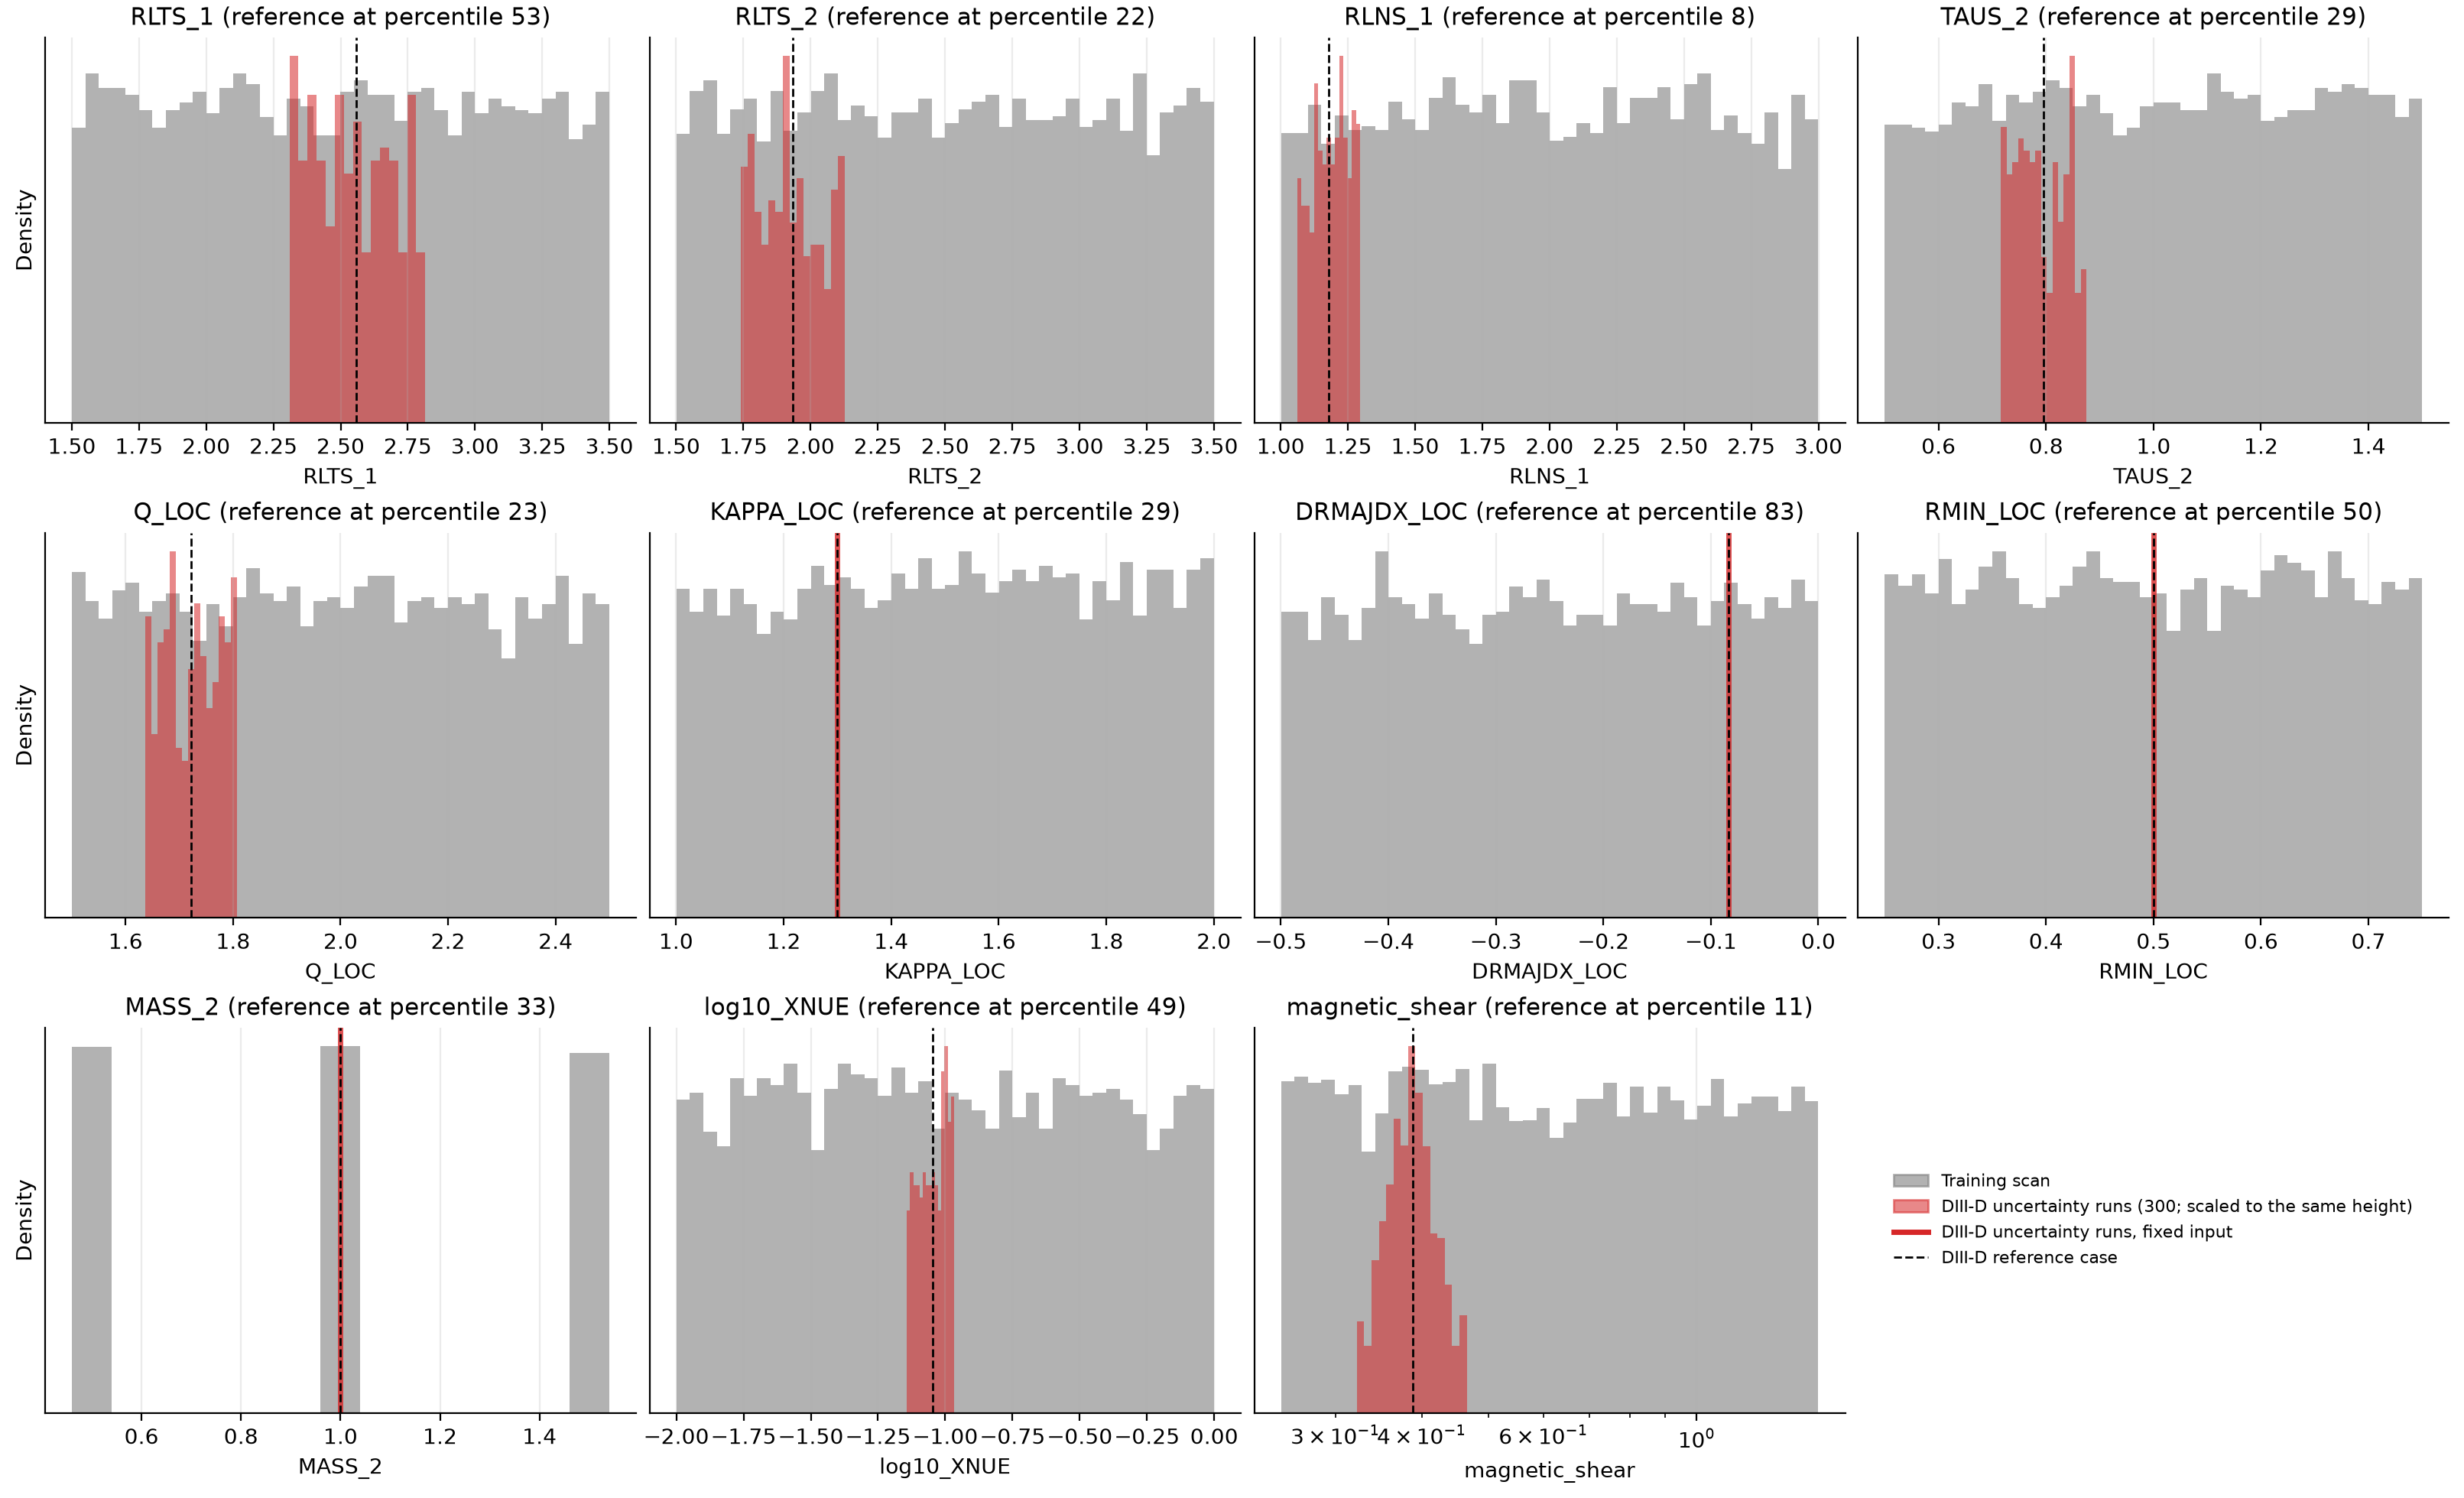
\includegraphics[width=0.95\linewidth]{figures/d3d_input_coverage.png}
  \caption{Distribution of each model input in the training scan (grey) and
    in the 300 DIII-D uncertainty runs (red, scaled to the same height). The
    dashed line is the DIII-D reference case and the title gives its
    percentile within the training scan. Inputs fixed in the DIII-D runs appear
    as a single red line.}
  \label{fig:d3d-inputs}
\end{figure}

\begin{table}[htbp]
  \centering
  \small
  \begin{tabular}{lrrrrrr}
    \toprule
                        & \multicolumn{3}{c}{Surrogate} & \multicolumn{3}{c}{TGLF (linear fit)}                                           \\
    \cmidrule(lr){2-4}\cmidrule(lr){5-7}
    Varied input        & $Q_i$                         & $Q_e$                                 & $\Gamma_e$ & $Q_i$ & $Q_e$ & $\Gamma_e$ \\
    \midrule
    \texttt{RLNS\_1}    & 5.7                           & 14.0                                  & 34.4       & 10.9  & 32.9  & 68.0       \\
    \texttt{RLTS\_2}    & 21.5                          & 6.7                                   & 11.3       & 31.5  & 3.7   & 8.2        \\
    All inputs together & 28.0                          & 22.9                                  & 41.4       & 42.3  & 44.8  & 80.0       \\
    \bottomrule
  \end{tabular}
  \caption{Flux uncertainty (half of the 5--95\% range, as a percentage of the
    mean flux) when one input has its error bar, and when all do. For TGLF,
    the per-input rows come from a straight-line fit to the 300 runs and the
    last row from the runs themselves.}
  \label{tab:d3d-sensitivity}
\end{table}

\subsection{Member-Disagreement Intervals}
\label{sec:disagreement-results}

The sections above report the quantile ensemble
(Section~\ref{sec:interval-methods}). This subsection reports the
15-network ensemble (Section~\ref{sec:disagreement-methods}), whose
intervals come from member disagreement.

On the test set its coverage was 91.2\%, 90.1\%, and 91.9\% for $Q_i$, $Q_e$,
and $\Gamma_e$. This is closer to the nominal 90\% than the quantile intervals
(Table~\ref{tab:coverage}), but it required multipliers fitted on validation
data, which the quantile intervals did not.

Its intervals also failed on some inputs. In the outside-range collisionality
group, ion-heat RMSE was 1.324 times the ordinary test value while the member
standard deviation was only 0.343 times as large, so the members agreed more
as the error grew. On the same 300 DIII-D input cases, its mean predicted
particle flux was 0.995 against TGLF's 0.483, the same direction of bias as the
quantile ensemble, despite 100\% interval coverage. The average interval width
was 3.85 in gyro-Bohm units. Broad intervals can contain the reference values
while the central prediction stays biased. The cause of this local bias has not
been established.

\subsection{Gradient-Boosted Bootstrap Ensemble: Coverage, Extrapolation, and DIII-D Propagation}
\label{sec:gbdt-uncertainty-results}

This subsection reports the 10-member bootstrap ensemble over the
gradient-boosted histogram-tree surrogate (Section~\ref{sec:gbdt-methods}), a
third, separately calibrated interval method evaluated on its own
\texttt{scan\_db} split (Section~\ref{sec:gbdt-results}).

On its 750 in-distribution test cases, the calibrated 90\% interval's
empirical coverage was 91.20\% for $Q_i$, 87.87\% for $Q_e$, and 86.80\% for
$\Gamma_e$ against a nominal target of 90\%, close to nominal for $Q_i$ but a
few points low for $Q_e$ and $\Gamma_e$. Predicted uncertainty correlated
positively with absolute error (Pearson $r = 0.662$, $0.611$, and $0.683$ for
$Q_i$, $Q_e$, and $\Gamma_e$), so wider bootstrap spread does track larger
error on held-out in-distribution cases, with the same caveat as
Section~\ref{sec:width-results} that this is a loose, not precise,
relationship.

We then evaluated the same ensemble, without retraining, on the nine
\texttt{scan\_db\_outside} sweeps described in
Section~\ref{sec:accuracy-results} and Table~\ref{tab:ood-sweeps}. Error grew
in eight of the nine groups relative to the matched in-distribution test
error, with the largest growth for $Q_i$ under \texttt{ood\_RLTS\_2}
($R/L_{Ti}$ swept to 3.5--5.0; mean absolute error rose from 16.80 to 83.94,
a 5.00$\times$ increase) and for $\Gamma_e$ under \texttt{ood\_RLN}
($R/L_n$ swept to 3.0--4.5; a 6.76$\times$ increase). The sole exception was
\texttt{ood\_XNUE}, where error fell below the in-distribution value for all
three fluxes, consistent with high collisionality suppressing trapped-electron-mode
and drift-wave turbulence toward zero transport. Ensemble spread grew in the
same direction but by much less than the error: for example, under
\texttt{ood\_RLTS\_2} the $Q_i$ error ratio was 5.00 while the corresponding
standard-deviation ratio was only 1.75. This mismatch has a structural cause.
Because decision trees partition the input space using axis-aligned cuts at
the training data's boundaries, a tree ensemble's predictions extrapolate as
piecewise-constant functions once a query falls outside the training bounding
box: every member keeps returning the value of whichever boundary leaf the
query lands in, so bootstrap resampling changes which leaf is selected far
less than it would change the true, unbounded physical flux. As a direct
consequence, calibrated 90\% coverage degraded substantially under
extrapolation, falling to 53.3\% for $Q_i$ under \texttt{ood\_RLTS\_2} and to
66.7\% for $Q_i$ and $\Gamma_e$ under \texttt{ood\_DRMAJDX\_LOC} ($\Delta'$
swept to $-0.75$--$-0.5$), the two lowest values among the 27 group-by-flux
combinations. The error bars widen on these out-of-range inputs, giving a
weak signal of elevated risk, but not enough to flag that the predictions
have become unreliable.

Finally, we propagated the same DIII-D reference-case input error bars used
in Section~\ref{sec:d3d-results} through this ensemble with a 10,000-draw
Monte Carlo sample, evaluated in 0.876\,s total (87.6\,$\mu$s per draw,
about 11,400 draws per second on one CPU core). The resulting $Q_i$
distribution had mean 3.56 and standard deviation 1.56 (a 43.7\% relative
spread, 90\% range $[1.20, 6.33]$); $Q_e$ had mean 5.21 and standard
deviation 1.08 (20.8\% relative spread, range $[3.46, 7.05]$); and $\Gamma_e$
had mean 0.55 and standard deviation 0.20 (35.5\% relative spread, range
$[0.24, 0.88]$). Measured against the 300 ground-truth TGLF runs at the same
input error bars, the surrogate's point predictions correlated well with TGLF
($r = 0.891$, $0.687$, and $0.742$ for $Q_i$, $Q_e$, and $\Gamma_e$), and the
calibrated 90\% interval around the matched 300-case predictions contained
the TGLF value in 100.0\%, 99.7\%, and 99.7\% of cases, wider than the
nominal 90\% target. A single-input sensitivity sweep, varying one input at a
time within its own error bar while holding the rest at the exact reference
values (Table~\ref{tab:gbdt-d3d-sensitivity}), shows that the dominant driver
differs by flux: $R/L_{Ti}$ (\texttt{RLTS\_2}) dominates the $Q_i$ spread,
collisionality $\nu_{ei}$ (\texttt{XNUE}) dominates the $Q_e$ spread, and the
density gradient $R/L_n$ (\texttt{RLNS}) dominates the $\Gamma_e$ spread.

\begin{table}[htbp]
  \centering
  \small
  \begin{tabular}{lrrr}
    \toprule
    Varied input (error bar)     & Std($Q_i$) & Std($Q_e$) & Std($\Gamma_e$) \\
    \midrule
    \texttt{RLTS\_1} ($\pm$10\%) & 0.228      & 0.532      & 0.083           \\
    \texttt{RLTS\_2} ($\pm$10\%) & 1.191      & 0.365      & 0.071           \\
    \texttt{RLNS} ($\pm$10\%)    & 0.146      & 0.443      & 0.137           \\
    \texttt{TAUS\_2} ($\pm$10\%) & 0.401      & 0.154      & 0.019           \\
    \texttt{XNUE} ($\pm$20\%)    & 0.752      & 0.651      & 0.024           \\
    \texttt{Q\_LOC} ($\pm$5\%)   & 0.289      & 0.325      & 0.093           \\
    \texttt{Q\_PRIME\_LOC} ($\pm$10\%) & 0.132 & 0.095     & 0.025           \\
    \bottomrule
  \end{tabular}
  \caption{Standard deviation induced in each flux (gyro-Bohm units) when a
    single DIII-D input is varied within its own measurement error bar
    (5,000 draws), holding all other inputs at their exact reference values.
    The largest entry in each column is the dominant single-input driver for
    that flux.}
  \label{tab:gbdt-d3d-sensitivity}
\end{table}

\section{Discussion, Limitations, and Remaining Work}
\label{sec:discussion}

These experiments show that representation and training choices can matter
as much as model complexity. Logarithmic collision frequency improved the
small-data linear fits. On the larger database, the MLP had the lowest error
and the fastest prediction of the models we compared, and the accuracy
ensemble improved on its baselines, although activation changes traded
accuracy across outputs. The uncertainty results add three findings. Interval
width follows how much training data is available, so the intervals show where
the surrogate is reliable. Error rises on inputs outside the training range,
but a narrow interval does not guarantee accuracy. And at the DIII-D reference
case the surrogate predicts higher fluxes than TGLF and responds less strongly
to the input errors. Sign errors, incorrect trends, and this local bias show
why average error and interval coverage alone are insufficient.

In practice, these results support using the surrogate for inputs inside the
dense part of the \texttt{scan\_db} range, where its intervals are narrow and
its error tends to be lower. Its predictions need checking against TGLF for
low-flux conditions, for inputs outside the training range, and for conditions
such as the DIII-D reference case that were not part of the training scan. A
wide interval is a useful warning in these cases, but a narrow one is not proof
that the prediction is accurate.

The conclusions remain limited by the small structured starter set,
exploratory model-family selection, prior test inspection, and reuse of
validation data for uncertainty calibration. The learning curves cover one
nested sequence. Because the experiments use different datasets and
procedures, they cannot establish one model ranking or determine whether
ensembles outperform the group's boosted trees or a matched single network.

\subsection{Planned Model-Comparison Experiments}

We intend to test whether expanding the ensemble improves prediction enough
to justify the additional training and inference cost. The 32-network model
described by \citet{meneghini2017} motivates studying member count as a design
choice. A controlled comparison will hold the architecture, training data,
and fitting procedure fixed while varying the number of members, including
a single-network reference. Our existing accuracy, quantile, and 15-network
ensembles (Table~\ref{tab:models}) do not isolate this effect, because they
differ in more than member count.

Other proposed experiments concern alternative transformations of the input
features, different network depths and widths, and separate ensembles for
$Q_i$, $Q_e$, and $\Gamma_e$ in place of the current shared three-output
networks. The input-transform comparisons will extend beyond the current
logarithmic collision-frequency representation. Learned transformations will
be fitted on training data only. These choices will be selected using
validation data and evaluated for each target, with computational cost
reported for the full predictor. We will consolidate the group's other models
under the same evaluation procedure and preserve new assessment cases from
further tuning.

\subsection{Planned DIII-D Database Study}

Our mentor's November 2 project plan provides a sequence for applying these
methods to a DIII-D database. The first stage is to run TGLF at 13 supplied
radial locations and verify the results against the reference answers. The
Task 4 handout then specifies 500--1,000 additional cases per team member,
spread across these radii. Five inputs are varied around each reference
condition: the two temperature gradients, shared density gradient,
temperature ratio, and collision frequency. The database will retain the
prescribed geometry at each radius and apply the stated cleaning rule for
negative heat-flux cases.

The next stages are to train a baseline and neural network for the three
fluxes, attach uncertainty estimates, and evaluate new input cases supplied
by the mentors. Learning curves using 500, 1,000, 2,000, and all available
training cases will examine whether errors continue to decrease, intervals
shrink, and some input regions remain poorly represented. The final comparison
will evaluate the broad \texttt{scan\_db} surrogate and the DIII-D-trained
surrogate on the same DIII-D test cases, assessing both accuracy and the
reliability of uncertainty estimates.

The plan also lists two possible extensions: comparing surrogate error with
the discrepancy between TGLF and nonlinear CGYRO outputs, and examining the
contributions of low- and high-wavenumber turbulence to electron heat flux.
These extensions are separate from the main comparison. Throughout the
study, the plan emphasizes correlated plasma inputs, data quality, uncertainty
estimates for every prediction, and flags for inputs outside the training
data. This work remains distinct from the completed experiments reported above.

\clearpage
\makereference
\bibliography{reference}
\bibliographystyle{style/dsc180bibstyle}
\end{document}
